\documentclass[twoside]{book}

% Packages required by doxygen
\usepackage{fixltx2e}
\usepackage{calc}
\usepackage{doxygen}
\usepackage[export]{adjustbox} % also loads graphicx
\usepackage{graphicx}
\usepackage[utf8]{inputenc}
\usepackage{makeidx}
\usepackage{multicol}
\usepackage{multirow}
\PassOptionsToPackage{warn}{textcomp}
\usepackage{textcomp}
\usepackage[nointegrals]{wasysym}
\usepackage[table]{xcolor}

% NLS support packages
\usepackage[french]{babel}

% Font selection
\usepackage[T1]{fontenc}
\usepackage[scaled=.90]{helvet}
\usepackage{courier}
\usepackage{amssymb}
\usepackage{sectsty}
\renewcommand{\familydefault}{\sfdefault}
\allsectionsfont{%
  \fontseries{bc}\selectfont%
  \color{darkgray}%
}
\renewcommand{\DoxyLabelFont}{%
  \fontseries{bc}\selectfont%
  \color{darkgray}%
}
\newcommand{\+}{\discretionary{\mbox{\scriptsize$\hookleftarrow$}}{}{}}

% Page & text layout
\usepackage{geometry}
\geometry{%
  a4paper,%
  top=2.5cm,%
  bottom=2.5cm,%
  left=2.5cm,%
  right=2.5cm%
}
\tolerance=750
\hfuzz=15pt
\hbadness=750
\setlength{\emergencystretch}{15pt}
\setlength{\parindent}{0cm}
\setlength{\parskip}{0.2cm}
\makeatletter
\renewcommand{\paragraph}{%
  \@startsection{paragraph}{4}{0ex}{-1.0ex}{1.0ex}{%
    \normalfont\normalsize\bfseries\SS@parafont%
  }%
}
\renewcommand{\subparagraph}{%
  \@startsection{subparagraph}{5}{0ex}{-1.0ex}{1.0ex}{%
    \normalfont\normalsize\bfseries\SS@subparafont%
  }%
}
\makeatother

% Headers & footers
\usepackage{fancyhdr}
\pagestyle{fancyplain}
\fancyhead[LE]{\fancyplain{}{\bfseries\thepage}}
\fancyhead[CE]{\fancyplain{}{}}
\fancyhead[RE]{\fancyplain{}{\bfseries\leftmark}}
\fancyhead[LO]{\fancyplain{}{\bfseries\rightmark}}
\fancyhead[CO]{\fancyplain{}{}}
\fancyhead[RO]{\fancyplain{}{\bfseries\thepage}}
\fancyfoot[LE]{\fancyplain{}{}}
\fancyfoot[CE]{\fancyplain{}{}}
\fancyfoot[RE]{\fancyplain{}{\bfseries\scriptsize Généré le Jeudi 4 Juin 2015 16\+:09\+:43 pour Projet Rythmique par Doxygen }}
\fancyfoot[LO]{\fancyplain{}{\bfseries\scriptsize Généré le Jeudi 4 Juin 2015 16\+:09\+:43 pour Projet Rythmique par Doxygen }}
\fancyfoot[CO]{\fancyplain{}{}}
\fancyfoot[RO]{\fancyplain{}{}}
\renewcommand{\footrulewidth}{0.4pt}
\renewcommand{\chaptermark}[1]{%
  \markboth{#1}{}%
}
\renewcommand{\sectionmark}[1]{%
  \markright{\thesection\ #1}%
}

% Indices & bibliography
\usepackage{natbib}
\usepackage[titles]{tocloft}
\setcounter{tocdepth}{3}
\setcounter{secnumdepth}{5}
\makeindex

% Hyperlinks (required, but should be loaded last)
\usepackage{ifpdf}
\ifpdf
  \usepackage[pdftex,pagebackref=true]{hyperref}
\else
  \usepackage[ps2pdf,pagebackref=true]{hyperref}
\fi
\hypersetup{%
  colorlinks=true,%
  linkcolor=blue,%
  citecolor=blue,%
  unicode%
}

% Custom commands
\newcommand{\clearemptydoublepage}{%
  \newpage{\pagestyle{empty}\cleardoublepage}%
}


%===== C O N T E N T S =====

\begin{document}

% Titlepage & ToC
\hypersetup{pageanchor=false,
             bookmarks=true,
             bookmarksnumbered=true,
             pdfencoding=unicode
            }
\pagenumbering{roman}
\begin{titlepage}
\vspace*{7cm}
\begin{center}%
{\Large Projet Rythmique }\\
\vspace*{1cm}
{\large Généré par Doxygen 1.8.9.1}\\
\vspace*{0.5cm}
{\small Jeudi 4 Juin 2015 16:09:43}\\
\end{center}
\end{titlepage}
\clearemptydoublepage
\tableofcontents
\clearemptydoublepage
\pagenumbering{arabic}
\hypersetup{pageanchor=true}

%--- Begin generated contents ---
\chapter{Documentation du Projet Rythmique}
\label{index}\hypertarget{index}{}\hypertarget{index_intro_sec}{}\section{Introduction}\label{index_intro_sec}
This is the introduction.\hypertarget{index_install_sec}{}\section{Installation}\label{index_install_sec}
\hypertarget{index_step1}{}\subsection{Step 1\+: Opening the box}\label{index_step1}
etc... 
\chapter{Index hiérarchique}
\section{Hiérarchie des classes}
Cette liste d\textquotesingle{}héritage est classée approximativement par ordre alphabétique \+:\begin{DoxyCompactList}
\item Mono\+Behaviour\begin{DoxyCompactList}
\item \contentsline{section}{Animation}{\pageref{class_animation}}{}
\item \contentsline{section}{Loop}{\pageref{class_loop}}{}
\item \contentsline{section}{Music}{\pageref{class_music}}{}
\item \contentsline{section}{Predef}{\pageref{class_predef}}{}
\item \contentsline{section}{Sound}{\pageref{class_sound}}{}
\end{DoxyCompactList}
\end{DoxyCompactList}

\chapter{Index des classes}
\section{Liste des classes}
Liste des classes, structures, unions et interfaces avec une brève description \+:\begin{DoxyCompactList}
\item\contentsline{section}{\hyperlink{class_animation}{Animation} \\*Cette classe implémente la partie graphique de l\textquotesingle{}application. Elle permet d\textquotesingle{}instancier des cylindres et des sphères, de les mettre en mouvement, etc ... }{\pageref{class_animation}}{}
\item\contentsline{section}{\hyperlink{class_loop}{Loop} \\*Cette classe permet de définir une boucle qui pourra contenir des sons. }{\pageref{class_loop}}{}
\item\contentsline{section}{\hyperlink{class_metronome}{Metronome} \\*Cette classe permet d\textquotesingle{}instancier un métronome. }{\pageref{class_metronome}}{}
\item\contentsline{section}{\hyperlink{class_music}{Music} \\*Classe principale de l\textquotesingle{}application. C\textquotesingle{}est elle qui possède un Fixed\+Update et qui met à jour tous les autres composants. C\textquotesingle{}est également dans cette classe que sont récuperés les events claviers. }{\pageref{class_music}}{}
\item\contentsline{section}{\hyperlink{class_sound}{Sound} \\*Un son est associé à un Audio\+Clip ce qui permet de jouer un son à l\textquotesingle{}appui de touches. }{\pageref{class_sound}}{}
\end{DoxyCompactList}

\chapter{Index des fichiers}
\section{Liste des fichiers}
Liste de tous les fichiers avec une brève description \+:\begin{DoxyCompactList}
\item\contentsline{section}{/\+Users/robin/\+Google Drive/\+Travail/\+S9/\+P\+R\+I/projet rythmique github/projet-\/unity/projet-\/rythmique/\+Projet-\/rythmique/\+Assets/\+Scripts/\hyperlink{_animation_8cs}{Animation.\+cs} }{\pageref{_animation_8cs}}{}
\item\contentsline{section}{/\+Users/robin/\+Google Drive/\+Travail/\+S9/\+P\+R\+I/projet rythmique github/projet-\/unity/projet-\/rythmique/\+Projet-\/rythmique/\+Assets/\+Scripts/\hyperlink{_documentation_8cs}{Documentation.\+cs} }{\pageref{_documentation_8cs}}{}
\item\contentsline{section}{/\+Users/robin/\+Google Drive/\+Travail/\+S9/\+P\+R\+I/projet rythmique github/projet-\/unity/projet-\/rythmique/\+Projet-\/rythmique/\+Assets/\+Scripts/\hyperlink{_loop_8cs}{Loop.\+cs} }{\pageref{_loop_8cs}}{}
\item\contentsline{section}{/\+Users/robin/\+Google Drive/\+Travail/\+S9/\+P\+R\+I/projet rythmique github/projet-\/unity/projet-\/rythmique/\+Projet-\/rythmique/\+Assets/\+Scripts/\hyperlink{_metronome_8cs}{Metronome.\+cs} }{\pageref{_metronome_8cs}}{}
\item\contentsline{section}{/\+Users/robin/\+Google Drive/\+Travail/\+S9/\+P\+R\+I/projet rythmique github/projet-\/unity/projet-\/rythmique/\+Projet-\/rythmique/\+Assets/\+Scripts/\hyperlink{_music_8cs}{Music.\+cs} }{\pageref{_music_8cs}}{}
\item\contentsline{section}{/\+Users/robin/\+Google Drive/\+Travail/\+S9/\+P\+R\+I/projet rythmique github/projet-\/unity/projet-\/rythmique/\+Projet-\/rythmique/\+Assets/\+Scripts/\hyperlink{_sound_8cs}{Sound.\+cs} }{\pageref{_sound_8cs}}{}
\end{DoxyCompactList}

\chapter{Documentation des classes}
\hypertarget{class_animation}{}\section{Référence de la classe Animation}
\label{class_animation}\index{Animation@{Animation}}


Cette classe implémente la partie graphique de l\textquotesingle{}application. Elle permet d\textquotesingle{}instancier des cylindres et des sphères, de les mettre en mouvement, etc ...  


Graphe d\textquotesingle{}héritage de Animation\+:\begin{figure}[H]
\begin{center}
\leavevmode
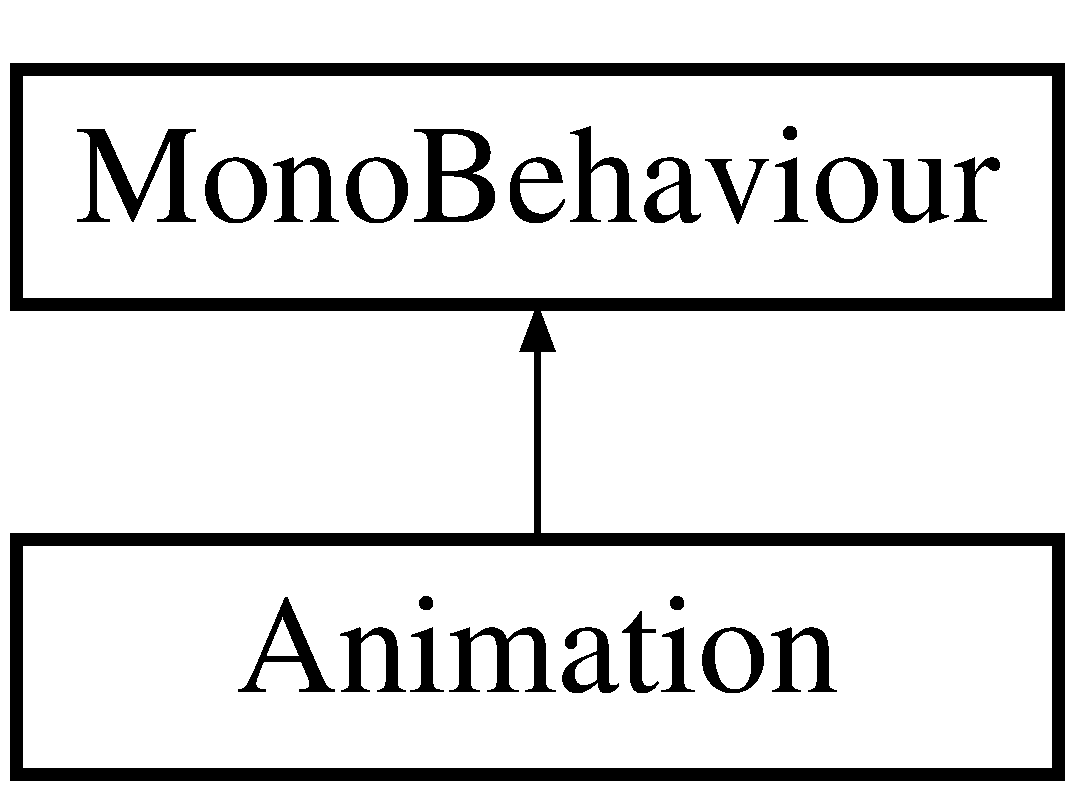
\includegraphics[height=2.000000cm]{class_animation}
\end{center}
\end{figure}
\subsection*{Fonctions membres publiques}
\begin{DoxyCompactItemize}
\item 
void \hyperlink{class_animation_ac57910012abaeb65ca0e626445eaefad}{Initialize} ()
\begin{DoxyCompactList}\small\item\em Initialisation de l\textquotesingle{}animation. \end{DoxyCompactList}\item 
void \hyperlink{class_animation_af22bd17e3ce0fa033af55bb9c6dd0d58}{Add\+Color} ()
\begin{DoxyCompactList}\small\item\em Construction du dictionnaire de couleurs. \end{DoxyCompactList}\item 
void \hyperlink{class_animation_a1dadb53b8ccec186d964a0450e78b47a}{draw\+Line} (float pos\+X, float pos\+Y, float pos\+Z)
\begin{DoxyCompactList}\small\item\em Dessin de la ligne rouge représentant le moment où le son va être joué. \end{DoxyCompactList}\item 
void \hyperlink{class_animation_a06d09825eeb89a1d53eff4a38b3ec6a7}{draw\+Sphere} (string color\+Name, int number, float pos\+X, float pos\+Y, float pos\+Z)
\begin{DoxyCompactList}\small\item\em Dessin des sphères représentants les sons. \end{DoxyCompactList}\item 
void \hyperlink{class_animation_a266bf2fda2038d9972419317aec73638}{make\+White} ()
\begin{DoxyCompactList}\small\item\em Permet de mettre tous les cylindres de liste de cylindres en blanc. \end{DoxyCompactList}\item 
void \hyperlink{class_animation_acf024d79e89180c5487b9059b2623ab5}{make\+Yellow} (Game\+Object cylinder)
\begin{DoxyCompactList}\small\item\em Permet de mettre un cylindre en jaune. \end{DoxyCompactList}\item 
void \hyperlink{class_animation_a42db90ac9b9ec3b2f3018380726f51ba}{draw\+Cylinder} (int number, float pos\+X, float pos\+Y, float pos\+Z)
\begin{DoxyCompactList}\small\item\em Dessin d\textquotesingle{}un cylindre. \end{DoxyCompactList}\item 
void \hyperlink{class_animation_ab70f71a9b180ece818d96c40cdcd7a42}{animate\+Cylinder} (float degree, int i)
\begin{DoxyCompactList}\small\item\em \hyperlink{class_animation}{Animation} des différents cylindres. \end{DoxyCompactList}\item 
void \hyperlink{class_animation_ae90a1074bf75c96180aa775e13162b6e}{camera\+Move} (float dist)
\begin{DoxyCompactList}\small\item\em Centrage de la caméra. \end{DoxyCompactList}\end{DoxyCompactItemize}
\subsection*{Attributs publics}
\begin{DoxyCompactItemize}
\item 
List$<$ Game\+Object $>$ \hyperlink{class_animation_a0d93aab7777651c0d98a8eb7c010dcf9}{cylinders} = new List$<$Game\+Object$>$()
\begin{DoxyCompactList}\small\item\em Liste des cylindres. \end{DoxyCompactList}\item 
List$<$ Game\+Object $>$ \hyperlink{class_animation_a96d77d0a4644c0a153f23c2f82ce50b9}{spheres} = new List$<$Game\+Object$>$()
\begin{DoxyCompactList}\small\item\em Liste des sphères. \end{DoxyCompactList}\end{DoxyCompactItemize}
\subsection*{Propriétés}
\begin{DoxyCompactItemize}
\item 
float \hyperlink{class_animation_a8d437d68fafe3193dc3b3bb652cfb4a8}{Cylinder\+Gap}\hspace{0.3cm}{\ttfamily  \mbox{[}get\mbox{]}}
\item 
List$<$ Game\+Object $>$ \hyperlink{class_animation_ada29c182dd9f01da8c5ee8f5afbf78cc}{Cylinders}\hspace{0.3cm}{\ttfamily  \mbox{[}get\mbox{]}}
\item 
List$<$ Game\+Object $>$ \hyperlink{class_animation_a54aef17d1bdc63728b435debc61a516f}{Spheres}\hspace{0.3cm}{\ttfamily  \mbox{[}get\mbox{]}}
\item 
float \hyperlink{class_animation_a2f2503f2087a873db779061cbf5ac188}{Size}\hspace{0.3cm}{\ttfamily  \mbox{[}get, set\mbox{]}}
\end{DoxyCompactItemize}
\subsection*{Attributs privés}
\begin{DoxyCompactItemize}
\item 
Game\+Object \hyperlink{class_animation_a51ca87e758a25805ddb89216570653c0}{container}
\begin{DoxyCompactList}\small\item\em Utiliser pour permet aux cylindres d\textquotesingle{}être le parent des sphères. \end{DoxyCompactList}\item 
Game\+Object \hyperlink{class_animation_adbb047fab7576bbef43eaf793cf090a6}{cyl}
\begin{DoxyCompactList}\small\item\em Game\+Object utilisé pour la création d\textquotesingle{}un cylindre. \end{DoxyCompactList}\item 
Game\+Object \hyperlink{class_animation_af7fc2df5c0ddc866cdbe608f31642dee}{sph}
\begin{DoxyCompactList}\small\item\em Game\+Object utulisé pour la création d\textquotesingle{}une sphères. \end{DoxyCompactList}\item 
Dictionary$<$ string, Color $>$ \hyperlink{class_animation_a294f170c53019f262d91e616410ae09c}{My\+Colors} = new Dictionary$<$string, Color$>$ ()
\begin{DoxyCompactList}\small\item\em Dictionnaire de couleur. \end{DoxyCompactList}\item 
float \hyperlink{class_animation_a89c2ae66fd6defd82f2f3ff5f82b4f4d}{size}
\begin{DoxyCompactList}\small\item\em Taille des cylindres et sphères. \end{DoxyCompactList}\item 
float \hyperlink{class_animation_a989c075387e746acc254fe2eeb83fb4c}{size\+Y} = 0.\+1f
\begin{DoxyCompactList}\small\item\em size\+Y = size $\ast$ size\+Ratio \end{DoxyCompactList}\item 
float \hyperlink{class_animation_a1e2704aeb83ffa433ed8e35f684fd39d}{cylinder\+Gap} = 0.\+3f
\begin{DoxyCompactList}\small\item\em Espace entre les cylindres. \end{DoxyCompactList}\item 
float \hyperlink{class_animation_a9c85a94c8eab9de9fa561bde4bd5b93b}{gap} = 0.\+2f
\begin{DoxyCompactList}\small\item\em Espace la barre d\textquotesingle{}action et les cylindres. \end{DoxyCompactList}\end{DoxyCompactItemize}


\subsection{Description détaillée}
Cette classe implémente la partie graphique de l\textquotesingle{}application. Elle permet d\textquotesingle{}instancier des cylindres et des sphères, de les mettre en mouvement, etc ... 



\subsection{Documentation des fonctions membres}
\hypertarget{class_animation_af22bd17e3ce0fa033af55bb9c6dd0d58}{}\index{Animation@{Animation}!Add\+Color@{Add\+Color}}
\index{Add\+Color@{Add\+Color}!Animation@{Animation}}
\subsubsection[{Add\+Color}]{\setlength{\rightskip}{0pt plus 5cm}void Animation.\+Add\+Color (
\begin{DoxyParamCaption}
{}
\end{DoxyParamCaption}
)}\label{class_animation_af22bd17e3ce0fa033af55bb9c6dd0d58}


Construction du dictionnaire de couleurs. 

\hypertarget{class_animation_ab70f71a9b180ece818d96c40cdcd7a42}{}\index{Animation@{Animation}!animate\+Cylinder@{animate\+Cylinder}}
\index{animate\+Cylinder@{animate\+Cylinder}!Animation@{Animation}}
\subsubsection[{animate\+Cylinder}]{\setlength{\rightskip}{0pt plus 5cm}void Animation.\+animate\+Cylinder (
\begin{DoxyParamCaption}
\item[{float}]{degree, }
\item[{int}]{i}
\end{DoxyParamCaption}
)}\label{class_animation_ab70f71a9b180ece818d96c40cdcd7a42}


\hyperlink{class_animation}{Animation} des différents cylindres. 


\begin{DoxyParams}{Paramètres}
{\em degree} & Rotation du cylindre.\\
\hline
{\em i} & Numéro du cylindre à faire tourner\\
\hline
\end{DoxyParams}
\hypertarget{class_animation_ae90a1074bf75c96180aa775e13162b6e}{}\index{Animation@{Animation}!camera\+Move@{camera\+Move}}
\index{camera\+Move@{camera\+Move}!Animation@{Animation}}
\subsubsection[{camera\+Move}]{\setlength{\rightskip}{0pt plus 5cm}void Animation.\+camera\+Move (
\begin{DoxyParamCaption}
\item[{float}]{dist}
\end{DoxyParamCaption}
)}\label{class_animation_ae90a1074bf75c96180aa775e13162b6e}


Centrage de la caméra. 


\begin{DoxyParams}{Paramètres}
{\em dist} & Somme de la largeur de tout les cylindres divisé par 2.\\
\hline
\end{DoxyParams}
\hypertarget{class_animation_a42db90ac9b9ec3b2f3018380726f51ba}{}\index{Animation@{Animation}!draw\+Cylinder@{draw\+Cylinder}}
\index{draw\+Cylinder@{draw\+Cylinder}!Animation@{Animation}}
\subsubsection[{draw\+Cylinder}]{\setlength{\rightskip}{0pt plus 5cm}void Animation.\+draw\+Cylinder (
\begin{DoxyParamCaption}
\item[{int}]{number, }
\item[{float}]{pos\+X, }
\item[{float}]{pos\+Y, }
\item[{float}]{pos\+Z}
\end{DoxyParamCaption}
)}\label{class_animation_a42db90ac9b9ec3b2f3018380726f51ba}


Dessin d\textquotesingle{}un cylindre. 


\begin{DoxyParams}{Paramètres}
{\em number} & Numéro du cylindre.\\
\hline
{\em pos\+X} & Position en X du cylindre.\\
\hline
{\em pos\+Y} & Position en Y du cylindre.\\
\hline
{\em pos\+Z} & Position en Z du cylindre.\\
\hline
\end{DoxyParams}
$<$ \mbox{[}A C\+O\+M\+P\+L\+E\+T\+E\+R\mbox{]} \hypertarget{class_animation_a1dadb53b8ccec186d964a0450e78b47a}{}\index{Animation@{Animation}!draw\+Line@{draw\+Line}}
\index{draw\+Line@{draw\+Line}!Animation@{Animation}}
\subsubsection[{draw\+Line}]{\setlength{\rightskip}{0pt plus 5cm}void Animation.\+draw\+Line (
\begin{DoxyParamCaption}
\item[{float}]{pos\+X, }
\item[{float}]{pos\+Y, }
\item[{float}]{pos\+Z}
\end{DoxyParamCaption}
)}\label{class_animation_a1dadb53b8ccec186d964a0450e78b47a}


Dessin de la ligne rouge représentant le moment où le son va être joué. 


\begin{DoxyParams}{Paramètres}
{\em pos\+X} & Position en X de la barre d\textquotesingle{}action\\
\hline
{\em pos\+Y} & Position en Y de la barre d\textquotesingle{}action\\
\hline
{\em pos\+Z} & Position en Z de la barre d\textquotesingle{}action\\
\hline
\end{DoxyParams}
\hypertarget{class_animation_a06d09825eeb89a1d53eff4a38b3ec6a7}{}\index{Animation@{Animation}!draw\+Sphere@{draw\+Sphere}}
\index{draw\+Sphere@{draw\+Sphere}!Animation@{Animation}}
\subsubsection[{draw\+Sphere}]{\setlength{\rightskip}{0pt plus 5cm}void Animation.\+draw\+Sphere (
\begin{DoxyParamCaption}
\item[{string}]{color\+Name, }
\item[{int}]{number, }
\item[{float}]{pos\+X, }
\item[{float}]{pos\+Y, }
\item[{float}]{pos\+Z}
\end{DoxyParamCaption}
)}\label{class_animation_a06d09825eeb89a1d53eff4a38b3ec6a7}


Dessin des sphères représentants les sons. 


\begin{DoxyParams}{Paramètres}
{\em color\+Name} & Couleur de la sphère.\\
\hline
{\em number} & Numéro de la sphère.\\
\hline
{\em pos\+X} & Position en X de la sphère.\\
\hline
{\em pos\+Y} & Position en Y de la sphère.\\
\hline
{\em pos\+Z} & Position en Z de la sphère.\\
\hline
\end{DoxyParams}
\hypertarget{class_animation_ac57910012abaeb65ca0e626445eaefad}{}\index{Animation@{Animation}!Initialize@{Initialize}}
\index{Initialize@{Initialize}!Animation@{Animation}}
\subsubsection[{Initialize}]{\setlength{\rightskip}{0pt plus 5cm}void Animation.\+Initialize (
\begin{DoxyParamCaption}
{}
\end{DoxyParamCaption}
)}\label{class_animation_ac57910012abaeb65ca0e626445eaefad}


Initialisation de l\textquotesingle{}animation. 

\hypertarget{class_animation_a266bf2fda2038d9972419317aec73638}{}\index{Animation@{Animation}!make\+White@{make\+White}}
\index{make\+White@{make\+White}!Animation@{Animation}}
\subsubsection[{make\+White}]{\setlength{\rightskip}{0pt plus 5cm}void Animation.\+make\+White (
\begin{DoxyParamCaption}
{}
\end{DoxyParamCaption}
)}\label{class_animation_a266bf2fda2038d9972419317aec73638}


Permet de mettre tous les cylindres de liste de cylindres en blanc. 

\hypertarget{class_animation_acf024d79e89180c5487b9059b2623ab5}{}\index{Animation@{Animation}!make\+Yellow@{make\+Yellow}}
\index{make\+Yellow@{make\+Yellow}!Animation@{Animation}}
\subsubsection[{make\+Yellow}]{\setlength{\rightskip}{0pt plus 5cm}void Animation.\+make\+Yellow (
\begin{DoxyParamCaption}
\item[{Game\+Object}]{cylinder}
\end{DoxyParamCaption}
)}\label{class_animation_acf024d79e89180c5487b9059b2623ab5}


Permet de mettre un cylindre en jaune. 


\begin{DoxyParams}{Paramètres}
{\em cylinder} & Cylindre à mettre en jaune.\\
\hline
\end{DoxyParams}


\subsection{Documentation des données membres}
\hypertarget{class_animation_a51ca87e758a25805ddb89216570653c0}{}\index{Animation@{Animation}!container@{container}}
\index{container@{container}!Animation@{Animation}}
\subsubsection[{container}]{\setlength{\rightskip}{0pt plus 5cm}Game\+Object Animation.\+container\hspace{0.3cm}{\ttfamily [private]}}\label{class_animation_a51ca87e758a25805ddb89216570653c0}


Utiliser pour permet aux cylindres d\textquotesingle{}être le parent des sphères. 

\hypertarget{class_animation_adbb047fab7576bbef43eaf793cf090a6}{}\index{Animation@{Animation}!cyl@{cyl}}
\index{cyl@{cyl}!Animation@{Animation}}
\subsubsection[{cyl}]{\setlength{\rightskip}{0pt plus 5cm}Game\+Object Animation.\+cyl\hspace{0.3cm}{\ttfamily [private]}}\label{class_animation_adbb047fab7576bbef43eaf793cf090a6}


Game\+Object utilisé pour la création d\textquotesingle{}un cylindre. 

\hypertarget{class_animation_a1e2704aeb83ffa433ed8e35f684fd39d}{}\index{Animation@{Animation}!cylinder\+Gap@{cylinder\+Gap}}
\index{cylinder\+Gap@{cylinder\+Gap}!Animation@{Animation}}
\subsubsection[{cylinder\+Gap}]{\setlength{\rightskip}{0pt plus 5cm}float Animation.\+cylinder\+Gap = 0.\+3f\hspace{0.3cm}{\ttfamily [private]}}\label{class_animation_a1e2704aeb83ffa433ed8e35f684fd39d}


Espace entre les cylindres. 

\hypertarget{class_animation_a0d93aab7777651c0d98a8eb7c010dcf9}{}\index{Animation@{Animation}!cylinders@{cylinders}}
\index{cylinders@{cylinders}!Animation@{Animation}}
\subsubsection[{cylinders}]{\setlength{\rightskip}{0pt plus 5cm}List$<$Game\+Object$>$ Animation.\+cylinders = new List$<$Game\+Object$>$()}\label{class_animation_a0d93aab7777651c0d98a8eb7c010dcf9}


Liste des cylindres. 

\hypertarget{class_animation_a9c85a94c8eab9de9fa561bde4bd5b93b}{}\index{Animation@{Animation}!gap@{gap}}
\index{gap@{gap}!Animation@{Animation}}
\subsubsection[{gap}]{\setlength{\rightskip}{0pt plus 5cm}float Animation.\+gap = 0.\+2f\hspace{0.3cm}{\ttfamily [private]}}\label{class_animation_a9c85a94c8eab9de9fa561bde4bd5b93b}


Espace la barre d\textquotesingle{}action et les cylindres. 

\hypertarget{class_animation_a294f170c53019f262d91e616410ae09c}{}\index{Animation@{Animation}!My\+Colors@{My\+Colors}}
\index{My\+Colors@{My\+Colors}!Animation@{Animation}}
\subsubsection[{My\+Colors}]{\setlength{\rightskip}{0pt plus 5cm}Dictionary$<$string, Color$>$ Animation.\+My\+Colors = new Dictionary$<$string, Color$>$ ()\hspace{0.3cm}{\ttfamily [private]}}\label{class_animation_a294f170c53019f262d91e616410ae09c}


Dictionnaire de couleur. 

\hypertarget{class_animation_a89c2ae66fd6defd82f2f3ff5f82b4f4d}{}\index{Animation@{Animation}!size@{size}}
\index{size@{size}!Animation@{Animation}}
\subsubsection[{size}]{\setlength{\rightskip}{0pt plus 5cm}float Animation.\+size\hspace{0.3cm}{\ttfamily [private]}}\label{class_animation_a89c2ae66fd6defd82f2f3ff5f82b4f4d}


Taille des cylindres et sphères. 

\hypertarget{class_animation_a989c075387e746acc254fe2eeb83fb4c}{}\index{Animation@{Animation}!size\+Y@{size\+Y}}
\index{size\+Y@{size\+Y}!Animation@{Animation}}
\subsubsection[{size\+Y}]{\setlength{\rightskip}{0pt plus 5cm}float Animation.\+size\+Y = 0.\+1f\hspace{0.3cm}{\ttfamily [private]}}\label{class_animation_a989c075387e746acc254fe2eeb83fb4c}


size\+Y = size $\ast$ size\+Ratio 

\hypertarget{class_animation_af7fc2df5c0ddc866cdbe608f31642dee}{}\index{Animation@{Animation}!sph@{sph}}
\index{sph@{sph}!Animation@{Animation}}
\subsubsection[{sph}]{\setlength{\rightskip}{0pt plus 5cm}Game\+Object Animation.\+sph\hspace{0.3cm}{\ttfamily [private]}}\label{class_animation_af7fc2df5c0ddc866cdbe608f31642dee}


Game\+Object utulisé pour la création d\textquotesingle{}une sphères. 

\hypertarget{class_animation_a96d77d0a4644c0a153f23c2f82ce50b9}{}\index{Animation@{Animation}!spheres@{spheres}}
\index{spheres@{spheres}!Animation@{Animation}}
\subsubsection[{spheres}]{\setlength{\rightskip}{0pt plus 5cm}List$<$Game\+Object$>$ Animation.\+spheres = new List$<$Game\+Object$>$()}\label{class_animation_a96d77d0a4644c0a153f23c2f82ce50b9}


Liste des sphères. 



\subsection{Documentation des propriétés}
\hypertarget{class_animation_a8d437d68fafe3193dc3b3bb652cfb4a8}{}\index{Animation@{Animation}!Cylinder\+Gap@{Cylinder\+Gap}}
\index{Cylinder\+Gap@{Cylinder\+Gap}!Animation@{Animation}}
\subsubsection[{Cylinder\+Gap}]{\setlength{\rightskip}{0pt plus 5cm}float Animation.\+Cylinder\+Gap\hspace{0.3cm}{\ttfamily [get]}}\label{class_animation_a8d437d68fafe3193dc3b3bb652cfb4a8}
\hypertarget{class_animation_ada29c182dd9f01da8c5ee8f5afbf78cc}{}\index{Animation@{Animation}!Cylinders@{Cylinders}}
\index{Cylinders@{Cylinders}!Animation@{Animation}}
\subsubsection[{Cylinders}]{\setlength{\rightskip}{0pt plus 5cm}List$<$Game\+Object$>$ Animation.\+Cylinders\hspace{0.3cm}{\ttfamily [get]}}\label{class_animation_ada29c182dd9f01da8c5ee8f5afbf78cc}
\hypertarget{class_animation_a2f2503f2087a873db779061cbf5ac188}{}\index{Animation@{Animation}!Size@{Size}}
\index{Size@{Size}!Animation@{Animation}}
\subsubsection[{Size}]{\setlength{\rightskip}{0pt plus 5cm}float Animation.\+Size\hspace{0.3cm}{\ttfamily [get]}, {\ttfamily [set]}}\label{class_animation_a2f2503f2087a873db779061cbf5ac188}
\hypertarget{class_animation_a54aef17d1bdc63728b435debc61a516f}{}\index{Animation@{Animation}!Spheres@{Spheres}}
\index{Spheres@{Spheres}!Animation@{Animation}}
\subsubsection[{Spheres}]{\setlength{\rightskip}{0pt plus 5cm}List$<$Game\+Object$>$ Animation.\+Spheres\hspace{0.3cm}{\ttfamily [get]}}\label{class_animation_a54aef17d1bdc63728b435debc61a516f}


La documentation de cette classe a été générée à partir du fichier suivant \+:\begin{DoxyCompactItemize}
\item 
/\+Users/robin/\+Google Drive/\+Travail/\+S9/\+P\+R\+I/projet rythmique github/projet-\/unity/projet-\/rythmique/\+Projet-\/rythmique/\+Assets/\+Scripts/\hyperlink{_animation_8cs}{Animation.\+cs}\end{DoxyCompactItemize}

\hypertarget{class_loop}{}\section{Référence de la classe Loop}
\label{class_loop}\index{Loop@{Loop}}


Cette classe permet de définir une boucle qui pourra contenir des sons.  


\subsection*{Fonctions membres publiques}
\begin{DoxyCompactItemize}
\item 
void \hyperlink{class_loop_a3a228a27bd11fd29c62845024654e68b}{play\+Sound} ()
\begin{DoxyCompactList}\small\item\em Fonction qui parcourt la liste des sons pour les jouer. \end{DoxyCompactList}\item 
float \hyperlink{class_loop_ac69e73a7f3b87ecdc51e3840505b6599}{Adjust\+Sound} (Game\+Object sph)
\begin{DoxyCompactList}\small\item\em Ajustement d\textquotesingle{}un son avec un autre son proche. \end{DoxyCompactList}\item 
void \hyperlink{class_loop_a728f506b8fb86bd3cc1701f8cd42b403}{Add\+Sound} (string title, float time=-\/1, float delay=0.\+0f)
\begin{DoxyCompactList}\small\item\em Ajout d\textquotesingle{}un son à une boucle. \end{DoxyCompactList}\item 
void \hyperlink{class_loop_afe51ea74b1e2bb59e3c22be8247134be}{Add\+Color} (string title, Game\+Object go)
\begin{DoxyCompactList}\small\item\em Ajoute les couleurs./// \end{DoxyCompactList}\end{DoxyCompactItemize}
\subsection*{Attributs publics}
\begin{DoxyCompactItemize}
\item 
List$<$ Game\+Object $>$ \hyperlink{class_loop_a49058954a754656c000691d0ea34d332}{spheres} = new List$<$Game\+Object$>$()
\begin{DoxyCompactList}\small\item\em Liste des sons de la boucle. \end{DoxyCompactList}\item 
List$<$ Audio\+Clip $>$ \hyperlink{class_loop_a900e93bdf5d703ce8bf4f12fa754e022}{clips} = new List$<$Audio\+Clip$>$()
\begin{DoxyCompactList}\small\item\em Liste des clips dans la boucle. \end{DoxyCompactList}\end{DoxyCompactItemize}
\subsection*{Propriétés}
\begin{DoxyCompactItemize}
\item 
float \hyperlink{class_loop_a50eeceb1774c7d9bb78f0b1c545010d2}{Loop\+Duration}\hspace{0.3cm}{\ttfamily  \mbox{[}get, set\mbox{]}}
\end{DoxyCompactItemize}
\subsection*{Fonctions membres privées}
\begin{DoxyCompactItemize}
\item 
void \hyperlink{class_loop_a9eeb1aa2e5cb39a0f3051b7dc8fc4fc2}{Awake} ()
\begin{DoxyCompactList}\small\item\em Awake this instance. \end{DoxyCompactList}\item 
void \hyperlink{class_loop_ae9848ead9ef01735696c2d954c1356ef}{Fixed\+Update} ()
\begin{DoxyCompactList}\small\item\em Fixeds the update. Utilise la fonction Play\+Soud pour jouer les sons. Calcul le temps actuel de la boucle (loop\+Time). \end{DoxyCompactList}\end{DoxyCompactItemize}
\subsection*{Attributs privés}
\begin{DoxyCompactItemize}
\item 
Audio\+Clip\mbox{[}$\,$\mbox{]} \hyperlink{class_loop_a1dfc5163d00ce897737c2a9bb95d72c3}{clip\+Array}
\begin{DoxyCompactList}\small\item\em Tableau contenant les audio\+Clips. \end{DoxyCompactList}\item 
float \hyperlink{class_loop_a5b85a1c3af3975aab929058d084929f0}{loop\+Duration}
\begin{DoxyCompactList}\small\item\em Durée de la boucle. \end{DoxyCompactList}\item 
float \hyperlink{class_loop_ab6f3df1dceea6e92a1728d8ad3558f4b}{loop\+Time} = 0.\+0f
\begin{DoxyCompactList}\small\item\em Temps courant de la boucle. \end{DoxyCompactList}\item 
float \hyperlink{class_loop_a483ac8b940665a7661559d82b9f8b3e5}{ratio}
\begin{DoxyCompactList}\small\item\em Rapport calculé pour avoir des secondes dans Unity. \end{DoxyCompactList}\item 
double \hyperlink{class_loop_a1e9897b50db8948891a1af99c7f354ca}{accuracy} = 5.\+0f
\item 
float \hyperlink{class_loop_a0db6a9a6439342876ec7eee9acf3a4bd}{marge} = 0.\+010f
\begin{DoxyCompactList}\small\item\em Marge défini pour l\textquotesingle{}ajustement des sons. \end{DoxyCompactList}\item 
Material \hyperlink{class_loop_ad2d1665b1488b64a26f42ed2ab7dc83a}{black}
\begin{DoxyCompactList}\small\item\em Définition du matériau Noir. \end{DoxyCompactList}\item 
Material \hyperlink{class_loop_abdff42bcd7fd2129d096263de28962ba}{blue}
\begin{DoxyCompactList}\small\item\em Définition du matériau Bleu. \end{DoxyCompactList}\item 
Material \hyperlink{class_loop_a081f72cca998dd79be5dfd7e27b126f4}{red}
\begin{DoxyCompactList}\small\item\em Définition du matériau Rouge. \end{DoxyCompactList}\item 
Material \hyperlink{class_loop_ad073115a8a8c600f326b875b2f8b6d35}{green}
\begin{DoxyCompactList}\small\item\em Définition du matériau Vert. \end{DoxyCompactList}\item 
Material \hyperlink{class_loop_ae76c0e46e59d56e3b602d597bceae38e}{neutre}
\begin{DoxyCompactList}\small\item\em Définition du matériau Neutre. \end{DoxyCompactList}\end{DoxyCompactItemize}


\subsection{Description détaillée}
Cette classe permet de définir une boucle qui pourra contenir des sons. 



Est dérivée de Mono\+Behaviour.



\subsection{Documentation des fonctions membres}
\hypertarget{class_loop_afe51ea74b1e2bb59e3c22be8247134be}{}\index{Loop@{Loop}!Add\+Color@{Add\+Color}}
\index{Add\+Color@{Add\+Color}!Loop@{Loop}}
\subsubsection[{Add\+Color}]{\setlength{\rightskip}{0pt plus 5cm}void Loop.\+Add\+Color (
\begin{DoxyParamCaption}
\item[{string}]{title, }
\item[{Game\+Object}]{go}
\end{DoxyParamCaption}
)\hspace{0.3cm}{\ttfamily [inline]}}\label{class_loop_afe51ea74b1e2bb59e3c22be8247134be}


Ajoute les couleurs./// 


\begin{DoxyParams}{Paramètres}
{\em title} & Titre du son.\\
\hline
{\em go} & Game\+Object associé au son, qui recevra la couleur.\\
\hline
\end{DoxyParams}
\hypertarget{class_loop_a728f506b8fb86bd3cc1701f8cd42b403}{}\index{Loop@{Loop}!Add\+Sound@{Add\+Sound}}
\index{Add\+Sound@{Add\+Sound}!Loop@{Loop}}
\subsubsection[{Add\+Sound}]{\setlength{\rightskip}{0pt plus 5cm}void Loop.\+Add\+Sound (
\begin{DoxyParamCaption}
\item[{string}]{title, }
\item[{float}]{time = {\ttfamily -\/1}, }
\item[{float}]{delay = {\ttfamily 0.0f}}
\end{DoxyParamCaption}
)\hspace{0.3cm}{\ttfamily [inline]}}\label{class_loop_a728f506b8fb86bd3cc1701f8cd42b403}


Ajout d\textquotesingle{}un son à une boucle. 


\begin{DoxyParams}{Paramètres}
{\em title} & Titre de l\textquotesingle{}Audio\+Clip à ajouter à la boucle.\\
\hline
{\em time} & Paramètre à fournir pour ajouter un son à un temps voulu.\\
\hline
{\em delay} & Décalage entre l\textquotesingle{}appui d\textquotesingle{}une touche et l\textquotesingle{}ajout d\textquotesingle{}un son.\\
\hline
\end{DoxyParams}
\hypertarget{class_loop_ac69e73a7f3b87ecdc51e3840505b6599}{}\index{Loop@{Loop}!Adjust\+Sound@{Adjust\+Sound}}
\index{Adjust\+Sound@{Adjust\+Sound}!Loop@{Loop}}
\subsubsection[{Adjust\+Sound}]{\setlength{\rightskip}{0pt plus 5cm}float Loop.\+Adjust\+Sound (
\begin{DoxyParamCaption}
\item[{Game\+Object}]{sph}
\end{DoxyParamCaption}
)\hspace{0.3cm}{\ttfamily [inline]}}\label{class_loop_ac69e73a7f3b87ecdc51e3840505b6599}


Ajustement d\textquotesingle{}un son avec un autre son proche. 

\begin{DoxyReturn}{Renvoie}
Retourne le temps ajusté (moyenne des deux sons proches).
\end{DoxyReturn}

\begin{DoxyParams}{Paramètres}
{\em sph} & Utilisation du game\+Object contenant le son à ajuster.\\
\hline
\end{DoxyParams}
\begin{DoxyRefDesc}{Bogue}
\item[\hyperlink{bug__bug000001}{Bogue}]Si on veut ajuster un son qui se trouve en fin de boucle alors l\textquotesingle{}ajustement ne va pas se faire en fin de boucle mais au milieu... ~\newline
 Explications \+:\end{DoxyRefDesc}
\begin{DoxyVerb}La boucle fait 5s:                                                                      |----------|
Un son est présent en fin de boucle :                                                   |---------S|
On ajuste avec un nouveau mais le temps que l'on appui il se situe en début de boucle : |S--------S|
Le nouveau son ajusté va se trouver en milieu de boucle :                               |----S-----|
\end{DoxyVerb}


\begin{DoxyRefDesc}{A faire}
\item[\hyperlink{todo__todo000001}{A faire}]Si le son à ajuster présent dans la liste est trop près de la fin de la boucle alors on ajuste en fin de boucle.\end{DoxyRefDesc}


Idée de code \+:

if ((Sspheres.\+Time+marge$>$loop\+Duration $\vert$$\vert$ Ssphere.\+Time+marge$>$loop\+Duration) \&\& (Sspheres.\+Time$<$loop\+Duration/2.\+0f $\vert$$\vert$ Ssphere.\+Time$<$loop\+Duration/2.\+0f) )\{ adjusted\+Time = ((Sspheres.\+Time+\+Ssphere.Time)-\/loop\+Duration)/2.0f; Destroy(spheres\mbox{[}i\mbox{]});\hypertarget{class_loop_a9eeb1aa2e5cb39a0f3051b7dc8fc4fc2}{}\index{Loop@{Loop}!Awake@{Awake}}
\index{Awake@{Awake}!Loop@{Loop}}
\subsubsection[{Awake}]{\setlength{\rightskip}{0pt plus 5cm}void Loop.\+Awake (
\begin{DoxyParamCaption}
{}
\end{DoxyParamCaption}
)\hspace{0.3cm}{\ttfamily [inline]}, {\ttfamily [private]}}\label{class_loop_a9eeb1aa2e5cb39a0f3051b7dc8fc4fc2}


Awake this instance. 

V\+E\+R\+I\+F\+I\+E\+R L\textquotesingle{}U\+T\+I\+L\+I\+T\+E D\+U R\+A\+T\+I\+O. \hypertarget{class_loop_ae9848ead9ef01735696c2d954c1356ef}{}\index{Loop@{Loop}!Fixed\+Update@{Fixed\+Update}}
\index{Fixed\+Update@{Fixed\+Update}!Loop@{Loop}}
\subsubsection[{Fixed\+Update}]{\setlength{\rightskip}{0pt plus 5cm}void Loop.\+Fixed\+Update (
\begin{DoxyParamCaption}
{}
\end{DoxyParamCaption}
)\hspace{0.3cm}{\ttfamily [inline]}, {\ttfamily [private]}}\label{class_loop_ae9848ead9ef01735696c2d954c1356ef}


Fixeds the update. Utilise la fonction Play\+Soud pour jouer les sons. Calcul le temps actuel de la boucle (loop\+Time). 

\hypertarget{class_loop_a3a228a27bd11fd29c62845024654e68b}{}\index{Loop@{Loop}!play\+Sound@{play\+Sound}}
\index{play\+Sound@{play\+Sound}!Loop@{Loop}}
\subsubsection[{play\+Sound}]{\setlength{\rightskip}{0pt plus 5cm}void Loop.\+play\+Sound (
\begin{DoxyParamCaption}
{}
\end{DoxyParamCaption}
)\hspace{0.3cm}{\ttfamily [inline]}}\label{class_loop_a3a228a27bd11fd29c62845024654e68b}


Fonction qui parcourt la liste des sons pour les jouer. 



\subsection{Documentation des données membres}
\hypertarget{class_loop_a1e9897b50db8948891a1af99c7f354ca}{}\index{Loop@{Loop}!accuracy@{accuracy}}
\index{accuracy@{accuracy}!Loop@{Loop}}
\subsubsection[{accuracy}]{\setlength{\rightskip}{0pt plus 5cm}double Loop.\+accuracy = 5.\+0f\hspace{0.3cm}{\ttfamily [private]}}\label{class_loop_a1e9897b50db8948891a1af99c7f354ca}
\hypertarget{class_loop_ad2d1665b1488b64a26f42ed2ab7dc83a}{}\index{Loop@{Loop}!black@{black}}
\index{black@{black}!Loop@{Loop}}
\subsubsection[{black}]{\setlength{\rightskip}{0pt plus 5cm}Material Loop.\+black\hspace{0.3cm}{\ttfamily [private]}}\label{class_loop_ad2d1665b1488b64a26f42ed2ab7dc83a}


Définition du matériau Noir. 

\hypertarget{class_loop_abdff42bcd7fd2129d096263de28962ba}{}\index{Loop@{Loop}!blue@{blue}}
\index{blue@{blue}!Loop@{Loop}}
\subsubsection[{blue}]{\setlength{\rightskip}{0pt plus 5cm}Material Loop.\+blue\hspace{0.3cm}{\ttfamily [private]}}\label{class_loop_abdff42bcd7fd2129d096263de28962ba}


Définition du matériau Bleu. 

\hypertarget{class_loop_a1dfc5163d00ce897737c2a9bb95d72c3}{}\index{Loop@{Loop}!clip\+Array@{clip\+Array}}
\index{clip\+Array@{clip\+Array}!Loop@{Loop}}
\subsubsection[{clip\+Array}]{\setlength{\rightskip}{0pt plus 5cm}Audio\+Clip \mbox{[}$\,$\mbox{]} Loop.\+clip\+Array\hspace{0.3cm}{\ttfamily [private]}}\label{class_loop_a1dfc5163d00ce897737c2a9bb95d72c3}


Tableau contenant les audio\+Clips. 

\hypertarget{class_loop_a900e93bdf5d703ce8bf4f12fa754e022}{}\index{Loop@{Loop}!clips@{clips}}
\index{clips@{clips}!Loop@{Loop}}
\subsubsection[{clips}]{\setlength{\rightskip}{0pt plus 5cm}List$<$Audio\+Clip$>$ Loop.\+clips = new List$<$Audio\+Clip$>$()}\label{class_loop_a900e93bdf5d703ce8bf4f12fa754e022}


Liste des clips dans la boucle. 

\hypertarget{class_loop_ad073115a8a8c600f326b875b2f8b6d35}{}\index{Loop@{Loop}!green@{green}}
\index{green@{green}!Loop@{Loop}}
\subsubsection[{green}]{\setlength{\rightskip}{0pt plus 5cm}Material Loop.\+green\hspace{0.3cm}{\ttfamily [private]}}\label{class_loop_ad073115a8a8c600f326b875b2f8b6d35}


Définition du matériau Vert. 

\hypertarget{class_loop_a5b85a1c3af3975aab929058d084929f0}{}\index{Loop@{Loop}!loop\+Duration@{loop\+Duration}}
\index{loop\+Duration@{loop\+Duration}!Loop@{Loop}}
\subsubsection[{loop\+Duration}]{\setlength{\rightskip}{0pt plus 5cm}float Loop.\+loop\+Duration\hspace{0.3cm}{\ttfamily [private]}}\label{class_loop_a5b85a1c3af3975aab929058d084929f0}


Durée de la boucle. 

\hypertarget{class_loop_ab6f3df1dceea6e92a1728d8ad3558f4b}{}\index{Loop@{Loop}!loop\+Time@{loop\+Time}}
\index{loop\+Time@{loop\+Time}!Loop@{Loop}}
\subsubsection[{loop\+Time}]{\setlength{\rightskip}{0pt plus 5cm}float Loop.\+loop\+Time = 0.\+0f\hspace{0.3cm}{\ttfamily [private]}}\label{class_loop_ab6f3df1dceea6e92a1728d8ad3558f4b}


Temps courant de la boucle. 

\hypertarget{class_loop_a0db6a9a6439342876ec7eee9acf3a4bd}{}\index{Loop@{Loop}!marge@{marge}}
\index{marge@{marge}!Loop@{Loop}}
\subsubsection[{marge}]{\setlength{\rightskip}{0pt plus 5cm}float Loop.\+marge = 0.\+010f\hspace{0.3cm}{\ttfamily [private]}}\label{class_loop_a0db6a9a6439342876ec7eee9acf3a4bd}


Marge défini pour l\textquotesingle{}ajustement des sons. 

\hypertarget{class_loop_ae76c0e46e59d56e3b602d597bceae38e}{}\index{Loop@{Loop}!neutre@{neutre}}
\index{neutre@{neutre}!Loop@{Loop}}
\subsubsection[{neutre}]{\setlength{\rightskip}{0pt plus 5cm}Material Loop.\+neutre\hspace{0.3cm}{\ttfamily [private]}}\label{class_loop_ae76c0e46e59d56e3b602d597bceae38e}


Définition du matériau Neutre. 

\hypertarget{class_loop_a483ac8b940665a7661559d82b9f8b3e5}{}\index{Loop@{Loop}!ratio@{ratio}}
\index{ratio@{ratio}!Loop@{Loop}}
\subsubsection[{ratio}]{\setlength{\rightskip}{0pt plus 5cm}float Loop.\+ratio\hspace{0.3cm}{\ttfamily [private]}}\label{class_loop_a483ac8b940665a7661559d82b9f8b3e5}


Rapport calculé pour avoir des secondes dans Unity. 

\hypertarget{class_loop_a081f72cca998dd79be5dfd7e27b126f4}{}\index{Loop@{Loop}!red@{red}}
\index{red@{red}!Loop@{Loop}}
\subsubsection[{red}]{\setlength{\rightskip}{0pt plus 5cm}Material Loop.\+red\hspace{0.3cm}{\ttfamily [private]}}\label{class_loop_a081f72cca998dd79be5dfd7e27b126f4}


Définition du matériau Rouge. 

\hypertarget{class_loop_a49058954a754656c000691d0ea34d332}{}\index{Loop@{Loop}!spheres@{spheres}}
\index{spheres@{spheres}!Loop@{Loop}}
\subsubsection[{spheres}]{\setlength{\rightskip}{0pt plus 5cm}List$<$Game\+Object$>$ Loop.\+spheres = new List$<$Game\+Object$>$()}\label{class_loop_a49058954a754656c000691d0ea34d332}


Liste des sons de la boucle. 



\subsection{Documentation des propriétés}
\hypertarget{class_loop_a50eeceb1774c7d9bb78f0b1c545010d2}{}\index{Loop@{Loop}!Loop\+Duration@{Loop\+Duration}}
\index{Loop\+Duration@{Loop\+Duration}!Loop@{Loop}}
\subsubsection[{Loop\+Duration}]{\setlength{\rightskip}{0pt plus 5cm}float Loop.\+Loop\+Duration\hspace{0.3cm}{\ttfamily [get]}, {\ttfamily [set]}}\label{class_loop_a50eeceb1774c7d9bb78f0b1c545010d2}


La documentation de cette classe a été générée à partir du fichier suivant \+:\begin{DoxyCompactItemize}
\item 
/\+Volumes/\+C\+L\+E R\+O\+B\+I\+N/projet-\/rythmique/\+Projet-\/rythmique/\+Assets/\+Scripts/\hyperlink{_loop_8cs}{Loop.\+cs}\end{DoxyCompactItemize}

\hypertarget{class_metronome}{}\section{Référence de la classe Metronome}
\label{class_metronome}\index{Metronome@{Metronome}}


Cette classe permet d\textquotesingle{}instancier un métronome.  


Graphe d\textquotesingle{}héritage de Metronome\+:\begin{figure}[H]
\begin{center}
\leavevmode
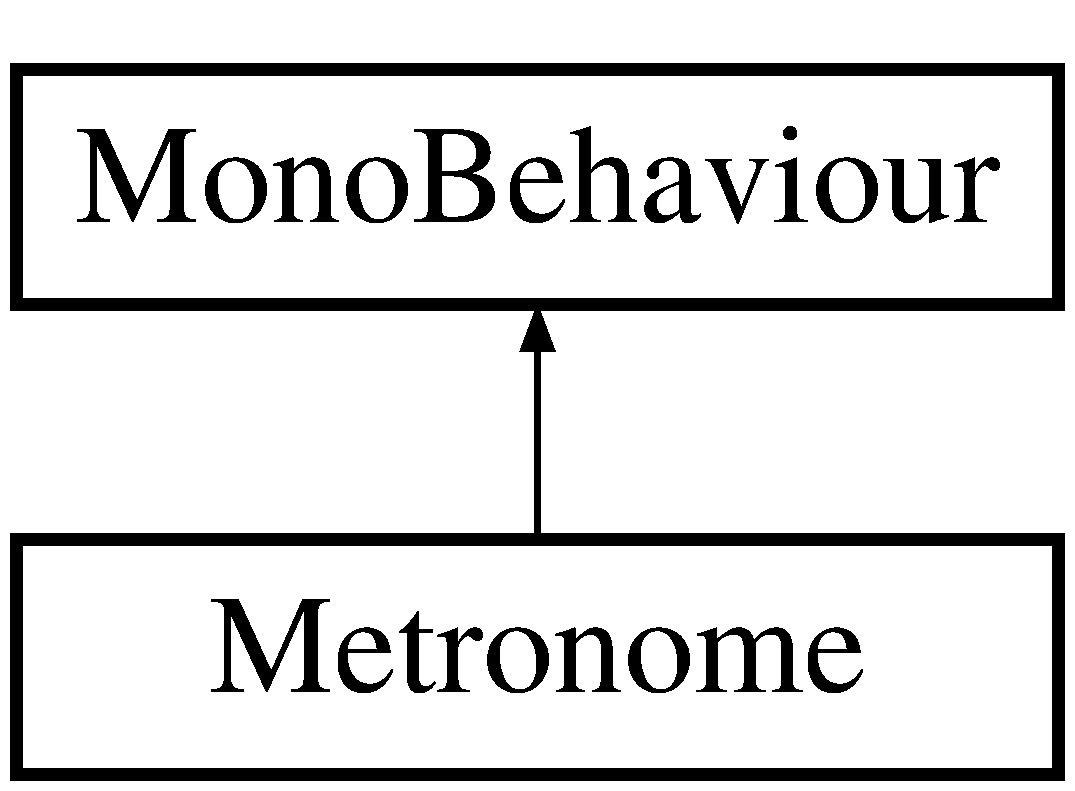
\includegraphics[height=2.000000cm]{class_metronome}
\end{center}
\end{figure}
\subsection*{Fonctions membres publiques}
\begin{DoxyCompactItemize}
\item 
void \hyperlink{class_metronome_a0189b04ace6a9f1b5bdb74cb8e3b20bc}{Initialize} ()
\begin{DoxyCompactList}\small\item\em Initialisation du métronome. \end{DoxyCompactList}\item 
void \hyperlink{class_metronome_a1bc290b5b41c27ab776b57214853e05b}{add\+Metronome} (int duree\+Metronome)
\begin{DoxyCompactList}\small\item\em Ajout des sons des sons du métronome. \end{DoxyCompactList}\item 
void \hyperlink{class_metronome_a51f41efee7a5e051c3a4c726f28149eb}{add\+Metronome\+Spheres} ()
\begin{DoxyCompactList}\small\item\em Ajout des sphères représentants les sons du métronome. \end{DoxyCompactList}\end{DoxyCompactItemize}
\subsection*{Attributs publics}
\begin{DoxyCompactItemize}
\item 
\hyperlink{class_music}{Music} \hyperlink{class_metronome_a9434e9e563d5b903c4a800d7529a0c9a}{music}
\begin{DoxyCompactList}\small\item\em Objet \hyperlink{class_music}{Music} qui permet d\textquotesingle{}ajouter une boucle à la liste de boucle ainsi que des sons à cette liste. \end{DoxyCompactList}\end{DoxyCompactItemize}
\subsection*{Propriétés}
\begin{DoxyCompactItemize}
\item 
bool \hyperlink{class_metronome_a2f04bf014bd373f690a955cce3298116}{Metronome\+Spheres}\hspace{0.3cm}{\ttfamily  \mbox{[}get, set\mbox{]}}
\end{DoxyCompactItemize}
\subsection*{Attributs privés}
\begin{DoxyCompactItemize}
\item 
bool \hyperlink{class_metronome_a3c3597941b45ceaebbe3b7f3b1a89faf}{metronome\+Spheres} = false
\begin{DoxyCompactList}\small\item\em Pour indiquer si toutes les sphères associées au métronome ont été dessinnes. \end{DoxyCompactList}\item 
int \hyperlink{class_metronome_a7e536279ddfa76b2aa0b77112ec0dd38}{metronome\+Spheres\+Count} = 0
\begin{DoxyCompactList}\small\item\em Nombre de sphères associées au métr. \end{DoxyCompactList}\end{DoxyCompactItemize}


\subsection{Description détaillée}
Cette classe permet d\textquotesingle{}instancier un métronome. 



\subsection{Documentation des fonctions membres}
\hypertarget{class_metronome_a1bc290b5b41c27ab776b57214853e05b}{}\index{Metronome@{Metronome}!add\+Metronome@{add\+Metronome}}
\index{add\+Metronome@{add\+Metronome}!Metronome@{Metronome}}
\subsubsection[{add\+Metronome}]{\setlength{\rightskip}{0pt plus 5cm}void Metronome.\+add\+Metronome (
\begin{DoxyParamCaption}
\item[{int}]{duree\+Metronome}
\end{DoxyParamCaption}
)}\label{class_metronome_a1bc290b5b41c27ab776b57214853e05b}


Ajout des sons des sons du métronome. 


\begin{DoxyParams}{Paramètres}
{\em duree\+Metronome} & Durée du métronome (en secondes).\\
\hline
\end{DoxyParams}
\hypertarget{class_metronome_a51f41efee7a5e051c3a4c726f28149eb}{}\index{Metronome@{Metronome}!add\+Metronome\+Spheres@{add\+Metronome\+Spheres}}
\index{add\+Metronome\+Spheres@{add\+Metronome\+Spheres}!Metronome@{Metronome}}
\subsubsection[{add\+Metronome\+Spheres}]{\setlength{\rightskip}{0pt plus 5cm}void Metronome.\+add\+Metronome\+Spheres (
\begin{DoxyParamCaption}
{}
\end{DoxyParamCaption}
)}\label{class_metronome_a51f41efee7a5e051c3a4c726f28149eb}


Ajout des sphères représentants les sons du métronome. 

\hypertarget{class_metronome_a0189b04ace6a9f1b5bdb74cb8e3b20bc}{}\index{Metronome@{Metronome}!Initialize@{Initialize}}
\index{Initialize@{Initialize}!Metronome@{Metronome}}
\subsubsection[{Initialize}]{\setlength{\rightskip}{0pt plus 5cm}void Metronome.\+Initialize (
\begin{DoxyParamCaption}
{}
\end{DoxyParamCaption}
)}\label{class_metronome_a0189b04ace6a9f1b5bdb74cb8e3b20bc}


Initialisation du métronome. 



\subsection{Documentation des données membres}
\hypertarget{class_metronome_a3c3597941b45ceaebbe3b7f3b1a89faf}{}\index{Metronome@{Metronome}!metronome\+Spheres@{metronome\+Spheres}}
\index{metronome\+Spheres@{metronome\+Spheres}!Metronome@{Metronome}}
\subsubsection[{metronome\+Spheres}]{\setlength{\rightskip}{0pt plus 5cm}bool Metronome.\+metronome\+Spheres = false\hspace{0.3cm}{\ttfamily [private]}}\label{class_metronome_a3c3597941b45ceaebbe3b7f3b1a89faf}


Pour indiquer si toutes les sphères associées au métronome ont été dessinnes. 

\hypertarget{class_metronome_a7e536279ddfa76b2aa0b77112ec0dd38}{}\index{Metronome@{Metronome}!metronome\+Spheres\+Count@{metronome\+Spheres\+Count}}
\index{metronome\+Spheres\+Count@{metronome\+Spheres\+Count}!Metronome@{Metronome}}
\subsubsection[{metronome\+Spheres\+Count}]{\setlength{\rightskip}{0pt plus 5cm}int Metronome.\+metronome\+Spheres\+Count = 0\hspace{0.3cm}{\ttfamily [private]}}\label{class_metronome_a7e536279ddfa76b2aa0b77112ec0dd38}


Nombre de sphères associées au métr. 

\hypertarget{class_metronome_a9434e9e563d5b903c4a800d7529a0c9a}{}\index{Metronome@{Metronome}!music@{music}}
\index{music@{music}!Metronome@{Metronome}}
\subsubsection[{music}]{\setlength{\rightskip}{0pt plus 5cm}{\bf Music} Metronome.\+music}\label{class_metronome_a9434e9e563d5b903c4a800d7529a0c9a}


Objet \hyperlink{class_music}{Music} qui permet d\textquotesingle{}ajouter une boucle à la liste de boucle ainsi que des sons à cette liste. 



\subsection{Documentation des propriétés}
\hypertarget{class_metronome_a2f04bf014bd373f690a955cce3298116}{}\index{Metronome@{Metronome}!Metronome\+Spheres@{Metronome\+Spheres}}
\index{Metronome\+Spheres@{Metronome\+Spheres}!Metronome@{Metronome}}
\subsubsection[{Metronome\+Spheres}]{\setlength{\rightskip}{0pt plus 5cm}bool Metronome.\+Metronome\+Spheres\hspace{0.3cm}{\ttfamily [get]}, {\ttfamily [set]}}\label{class_metronome_a2f04bf014bd373f690a955cce3298116}


La documentation de cette classe a été générée à partir du fichier suivant \+:\begin{DoxyCompactItemize}
\item 
/\+Users/robin/\+Google Drive/\+Travail/\+S9/\+P\+R\+I/projet rythmique github/projet-\/unity/projet-\/rythmique/\+Projet-\/rythmique/\+Assets/\+Scripts/\hyperlink{_metronome_8cs}{Metronome.\+cs}\end{DoxyCompactItemize}

\hypertarget{class_music}{}\section{Référence de la classe Music}
\label{class_music}\index{Music@{Music}}


Classe principale de l\textquotesingle{}application. C\textquotesingle{}est elle qui possède un Fixed\+Update et qui met à jour tous les autres composants. C\textquotesingle{}est également dans cette classe que sont récuperés les events claviers. La ligne rouge représente le moment ou les sons vont etre joués. Les cylindres représentent les boucles. Les sphères représentent les sons.  


\subsection*{Fonctions membres publiques}
\begin{DoxyCompactItemize}
\item 
void \hyperlink{class_music_a25d6adb92e3f3b05b996537d467a29f2}{Update\+Array} (int index=-\/1)
\begin{DoxyCompactList}\small\item\em Met à jour la liste des boucles. \end{DoxyCompactList}\item 
void \hyperlink{class_music_a3c969affd4d6d160a668e5fe33bec756}{Make\+Yellow} (Game\+Object go)
\begin{DoxyCompactList}\small\item\em Met en surbrillance la boucle sélectionnée. \end{DoxyCompactList}\item 
void \hyperlink{class_music_a118396d7b9526c5111f3d8d0e1f55c0d}{Destroy\+Loop} ()
\begin{DoxyCompactList}\small\item\em Détruit la boucle sélectionnée. \end{DoxyCompactList}\item 
void \hyperlink{class_music_afcef8e50a31bccf2cb425cfa851322d5}{Replace} (int select)
\begin{DoxyCompactList}\small\item\em Re-\/positionne les boucles après une suppression. \end{DoxyCompactList}\item 
void \hyperlink{class_music_ab103b2b4b594c28a547c5c44c4736390}{Add\+Loop} ()
\begin{DoxyCompactList}\small\item\em Ajoute des boucles. \end{DoxyCompactList}\item 
void \hyperlink{class_music_aecc7789c2058cbd454e28abef95a5f7e}{Camera\+Move} ()
\begin{DoxyCompactList}\small\item\em Repositionnement de la caméra. \end{DoxyCompactList}\end{DoxyCompactItemize}
\subsection*{Attributs publics}
\begin{DoxyCompactItemize}
\item 
List$<$ Game\+Object $>$ \hyperlink{class_music_ac34fdcf5a15ce705117105b68a72974d}{loops} = new List$<$Game\+Object$>$()
\begin{DoxyCompactList}\small\item\em Liste des boucles. \end{DoxyCompactList}\item 
Audio\+Source \hyperlink{class_music_ad7980e82c9bb7fc27ce15affbc4ef267}{audio\+Source}
\begin{DoxyCompactList}\small\item\em Objet \href{http://docs.unity3d.com/ScriptReference/AudioSource.html}{\tt Audio\+Source} qui permet de jouer un son. \end{DoxyCompactList}\item 
int \hyperlink{class_music_a2c0e87848bf12c5f29e62f22556f0bb0}{pressable\+Time} = 20
\end{DoxyCompactItemize}
\subsection*{Propriétés}
\begin{DoxyCompactItemize}
\item 
float \hyperlink{class_music_a20bb244d5d40d5848201077b577b0111}{Duration\+Time}\hspace{0.3cm}{\ttfamily  \mbox{[}get, set\mbox{]}}
\item 
int \hyperlink{class_music_a08b2e446def0d17e713d4f723811b3be}{Loop\+Selected}\hspace{0.3cm}{\ttfamily  \mbox{[}get\mbox{]}}
\item 
float \hyperlink{class_music_a215cbe531ec3578d7c5a06305b7e7873}{Bpm}\hspace{0.3cm}{\ttfamily  \mbox{[}get, set\mbox{]}}
\item 
float \hyperlink{class_music_a84523fd3eb5ec2fa076d69dd0fd18373}{Mesure}\hspace{0.3cm}{\ttfamily  \mbox{[}get, set\mbox{]}}
\end{DoxyCompactItemize}
\subsection*{Fonctions membres privées}
\begin{DoxyCompactItemize}
\item 
static void \hyperlink{class_music_a69b2158924c1cf3b72d8ad0aa31169b6}{wiimote\+\_\+start} ()
\item 
static void \hyperlink{class_music_ad87bc9d22b95c82090707ddc53ed5da8}{wiimote\+\_\+stop} ()
\item 
static int \hyperlink{class_music_a40595d7c6af2acb00fb2bb7841cb5f67}{wiimote\+\_\+count} ()
\item 
static bool \hyperlink{class_music_a0da54a9b72517be2ef96b56817730de4}{wiimote\+\_\+get\+Button\+A} (int which)
\item 
static bool \hyperlink{class_music_afa8c29f119c92db2e15df93fadb11008}{wiimote\+\_\+get\+Button\+B} (int which)
\item 
static byte \hyperlink{class_music_aee0db5bd6d8dcda6638368322eee4c85}{wiimote\+\_\+get\+Acc\+X} (int which)
\item 
static byte \hyperlink{class_music_a3a575f1623e1d8f08f9ef6a0fa3c0971}{wiimote\+\_\+get\+Acc\+Y} (int which)
\item 
static byte \hyperlink{class_music_a98817ef086d8628dbefb97c6dcc16784}{wiimote\+\_\+get\+Acc\+Z} (int which)
\item 
static float \hyperlink{class_music_acb804430cb256e5eed4c2f25e9792241}{wiimote\+\_\+get\+Roll} (int which)
\item 
static float \hyperlink{class_music_ab6d783cc9a08de26e36401ecefd0169f}{wiimote\+\_\+get\+Pitch} (int which)
\item 
static float \hyperlink{class_music_a8671f54d1c3d75b602c79e6b39c9707a}{wiimote\+\_\+get\+Yaw} (int which)
\item 
static bool \hyperlink{class_music_abe16123b93a805449f5125f3a461c704}{wiimote\+\_\+get\+Button\+Up} (int which)
\item 
static bool \hyperlink{class_music_a2684a38f892873250a4b720434c1a548}{wiimote\+\_\+get\+Button\+Left} (int which)
\item 
static bool \hyperlink{class_music_a4d3a8be82426aede2dcb42cd2618e93d}{wiimote\+\_\+get\+Button\+Right} (int which)
\item 
static bool \hyperlink{class_music_a7c5e9399a60e57bebf5c2e18b54ef499}{wiimote\+\_\+get\+Button\+Down} (int which)
\item 
static bool \hyperlink{class_music_a835f4686d6c9f04048ac82846d80c68d}{wiimote\+\_\+get\+Button1} (int which)
\item 
static bool \hyperlink{class_music_a159e2b41593b313b806b1fa75855a3b1}{wiimote\+\_\+get\+Button2} (int which)
\item 
static bool \hyperlink{class_music_afdd08708b534b7010afccc75124d8046}{wiimote\+\_\+get\+Button\+Plus} (int which)
\item 
static bool \hyperlink{class_music_a86a3c5ae8040d1c655a595ca23c61c33}{wiimote\+\_\+get\+Button\+Minus} (int which)
\item 
static bool \hyperlink{class_music_a24b68dad0f9ae028714d3106c748eda4}{wiimote\+\_\+get\+Button\+Home} (int which)
\item 
void \hyperlink{class_music_a88677b5b17d7881742cf8d0e23ac8207}{Start} ()
\item 
void \hyperlink{class_music_a57440cf9285a10dee627479fa0b7a3aa}{Fixed\+Update} ()
\item 
void \hyperlink{class_music_acb4d0b5d2b535f89fd14f1886baab776}{unable\+Press\+Key} ()
\begin{DoxyCompactList}\small\item\em Cette fonction permet d\textquotesingle{}empecher l\textquotesingle{}appuie sur une touche de la wii pendant un temps \textquotesingle{}pressable\+Time\textquotesingle{} afin de ne pas ajouter un son à chaque update si on reste appuyer sur un bouton de la Wii Remote. \end{DoxyCompactList}\item 
void \hyperlink{class_music_a034233438c74e4b0d6f1fecf5de6cacb}{On\+G\+U\+I} ()
\begin{DoxyCompactList}\small\item\em Dessine la fenetre graphique \end{DoxyCompactList}\item 
void \hyperlink{class_music_a67cf059d4e7f913a246a06e53d177e6c}{draw\+G\+U\+I} (int id)
\begin{DoxyCompactList}\small\item\em Dessine les boutons et récupère les événements associés. \end{DoxyCompactList}\item 
void \hyperlink{class_music_a6bcab145b7a68dac28bed9bc32affc44}{get\+Input\+Wiimote} (int which)
\begin{DoxyCompactList}\small\item\em Recupère les appuis sur les boutons de la wiimote. \end{DoxyCompactList}\item 
bool \hyperlink{class_music_a09593624eba620da5d6cbb09d6e2e845}{play\+Sound\+With\+Movement} (String son)
\item 
void \hyperlink{class_music_a063497fdbf5be69712dc08866e0e2ea5}{get\+Input} ()
\begin{DoxyCompactList}\small\item\em Lit les inputs clavier. \end{DoxyCompactList}\end{DoxyCompactItemize}
\subsection*{Attributs privés}
\begin{DoxyCompactItemize}
\item 
Game\+Object \hyperlink{class_music_a1507118c48dd86cf0cc02e35e9a878d2}{line}
\begin{DoxyCompactList}\small\item\em La ligne. \end{DoxyCompactList}\item 
Vector3 \hyperlink{class_music_a8dee10ad61d1260dc55195c7a7c50d7c}{pos\+Line}
\begin{DoxyCompactList}\small\item\em Position de la ligne. \end{DoxyCompactList}\item 
Game\+Object \hyperlink{class_music_ad8b992250bd9ff84988adc7c0091c321}{loop}
\begin{DoxyCompactList}\small\item\em Le cylindre. \end{DoxyCompactList}\item 
\hyperlink{class_predef}{Predef} \hyperlink{class_music_a23d19ec4b266573443920e3dacc9bd93}{predef}
\begin{DoxyCompactList}\small\item\em Instance de \hyperlink{class_predef}{Predef} qui sert à accéder aux boucles prédéfinies. \end{DoxyCompactList}\item 
Material \hyperlink{class_music_acf7deb58e516a37db39d3c9883d6034e}{yellow}
\begin{DoxyCompactList}\small\item\em Définition du matériau Jaune. \end{DoxyCompactList}\item 
Material \hyperlink{class_music_ac4412a8635c49f90692e3683931c0343}{neutre}
\begin{DoxyCompactList}\small\item\em Définition du matériau Neutre. \end{DoxyCompactList}\item 
float \hyperlink{class_music_ae4014f55d10343673bbf00004ebaaf31}{duration\+Time}
\begin{DoxyCompactList}\small\item\em Durée de la boucle qui va être créée. \end{DoxyCompactList}\item 
int \hyperlink{class_music_a89ea80578a05f37ffefe4f83d6be0425}{loop\+Number} = 0
\begin{DoxyCompactList}\small\item\em Numéro de la boucle qui va être créée. \end{DoxyCompactList}\item 
int \hyperlink{class_music_a314e1e14f9b0f2fc88672df0a54ceda2}{loop\+Selected} = -\/1
\begin{DoxyCompactList}\small\item\em Boucle selectionnée (en jaune). \end{DoxyCompactList}\item 
float \hyperlink{class_music_a32f83f56e3522b34faf524ef322459e7}{bpm} = 0.\+0f
\begin{DoxyCompactList}\small\item\em Nombre de B\+P\+M (battements par minute). \end{DoxyCompactList}\item 
float \hyperlink{class_music_adf436d51d0b5be109beae967b4d34522}{mesure} = 0.\+0f
\begin{DoxyCompactList}\small\item\em Nombre de mesure. \end{DoxyCompactList}\item 
String \hyperlink{class_music_a937e074ddcaba7ed3666cf872c94d97f}{wii\+\_\+display}
\item 
bool \hyperlink{class_music_ab653d0747a20992b8f891361ff75c2fc}{A}
\item 
bool \hyperlink{class_music_a16991bd6f416f0fe945e89d7d480cad6}{B}
\item 
int \hyperlink{class_music_acb9bb6d52e75b11d305be2a2ae180cb5}{X}
\item 
int \hyperlink{class_music_af45a2d376fdee07df8fc263f17e940b5}{Y}
\item 
int \hyperlink{class_music_ac55cf30eb31695f3b6ec7ace7a8abb19}{Z}
\item 
float \hyperlink{class_music_a2008a64ad37c7a232a8c206d7acdbd0f}{R}
\item 
float \hyperlink{class_music_a8811033babcd7646e477060f69d578e6}{P}
\item 
float \hyperlink{class_music_acd36d67bfd91798211295d45ef911c34}{W}
\item 
bool \hyperlink{class_music_a6525acdf11a00376a98d5178ab822886}{is\+Pressable} = true
\item 
int \hyperlink{class_music_a4d9b6dba41b560393edf85a675e8a84f}{nb\+Of\+Wiimote} = 0
\item 
bool \hyperlink{class_music_a207d2cf72a65ec7a1e4ce02e3cfd29b9}{cond\+Inf} = false
\item 
bool \hyperlink{class_music_aeeb6f3c67f4b24bb83aaecf68075f51b}{cond\+Sup} = false
\end{DoxyCompactItemize}


\subsection{Description détaillée}
Classe principale de l\textquotesingle{}application. C\textquotesingle{}est elle qui possède un Fixed\+Update et qui met à jour tous les autres composants. C\textquotesingle{}est également dans cette classe que sont récuperés les events claviers. La ligne rouge représente le moment ou les sons vont etre joués. Les cylindres représentent les boucles. Les sphères représentent les sons. 



Est dérivée de Mono\+Behaviour.



\subsection{Documentation des fonctions membres}
\hypertarget{class_music_ab103b2b4b594c28a547c5c44c4736390}{}\index{Music@{Music}!Add\+Loop@{Add\+Loop}}
\index{Add\+Loop@{Add\+Loop}!Music@{Music}}
\subsubsection[{Add\+Loop}]{\setlength{\rightskip}{0pt plus 5cm}void Music.\+Add\+Loop (
\begin{DoxyParamCaption}
{}
\end{DoxyParamCaption}
)\hspace{0.3cm}{\ttfamily [inline]}}\label{class_music_ab103b2b4b594c28a547c5c44c4736390}


Ajoute des boucles. 

\hypertarget{class_music_aecc7789c2058cbd454e28abef95a5f7e}{}\index{Music@{Music}!Camera\+Move@{Camera\+Move}}
\index{Camera\+Move@{Camera\+Move}!Music@{Music}}
\subsubsection[{Camera\+Move}]{\setlength{\rightskip}{0pt plus 5cm}void Music.\+Camera\+Move (
\begin{DoxyParamCaption}
{}
\end{DoxyParamCaption}
)\hspace{0.3cm}{\ttfamily [inline]}}\label{class_music_aecc7789c2058cbd454e28abef95a5f7e}


Repositionnement de la caméra. 

\hypertarget{class_music_a118396d7b9526c5111f3d8d0e1f55c0d}{}\index{Music@{Music}!Destroy\+Loop@{Destroy\+Loop}}
\index{Destroy\+Loop@{Destroy\+Loop}!Music@{Music}}
\subsubsection[{Destroy\+Loop}]{\setlength{\rightskip}{0pt plus 5cm}void Music.\+Destroy\+Loop (
\begin{DoxyParamCaption}
{}
\end{DoxyParamCaption}
)\hspace{0.3cm}{\ttfamily [inline]}}\label{class_music_a118396d7b9526c5111f3d8d0e1f55c0d}


Détruit la boucle sélectionnée. 

\hypertarget{class_music_a67cf059d4e7f913a246a06e53d177e6c}{}\index{Music@{Music}!draw\+G\+U\+I@{draw\+G\+U\+I}}
\index{draw\+G\+U\+I@{draw\+G\+U\+I}!Music@{Music}}
\subsubsection[{draw\+G\+U\+I}]{\setlength{\rightskip}{0pt plus 5cm}void Music.\+draw\+G\+U\+I (
\begin{DoxyParamCaption}
\item[{int}]{id}
\end{DoxyParamCaption}
)\hspace{0.3cm}{\ttfamily [inline]}, {\ttfamily [private]}}\label{class_music_a67cf059d4e7f913a246a06e53d177e6c}


Dessine les boutons et récupère les événements associés. 


\begin{DoxyParams}{Paramètres}
{\em id} & Identifiant de la fenetre.\\
\hline
\end{DoxyParams}
\hypertarget{class_music_a57440cf9285a10dee627479fa0b7a3aa}{}\index{Music@{Music}!Fixed\+Update@{Fixed\+Update}}
\index{Fixed\+Update@{Fixed\+Update}!Music@{Music}}
\subsubsection[{Fixed\+Update}]{\setlength{\rightskip}{0pt plus 5cm}void Music.\+Fixed\+Update (
\begin{DoxyParamCaption}
{}
\end{DoxyParamCaption}
)\hspace{0.3cm}{\ttfamily [inline]}, {\ttfamily [private]}}\label{class_music_a57440cf9285a10dee627479fa0b7a3aa}
\hypertarget{class_music_a063497fdbf5be69712dc08866e0e2ea5}{}\index{Music@{Music}!get\+Input@{get\+Input}}
\index{get\+Input@{get\+Input}!Music@{Music}}
\subsubsection[{get\+Input}]{\setlength{\rightskip}{0pt plus 5cm}void Music.\+get\+Input (
\begin{DoxyParamCaption}
{}
\end{DoxyParamCaption}
)\hspace{0.3cm}{\ttfamily [inline]}, {\ttfamily [private]}}\label{class_music_a063497fdbf5be69712dc08866e0e2ea5}


Lit les inputs clavier. 

\hypertarget{class_music_a6bcab145b7a68dac28bed9bc32affc44}{}\index{Music@{Music}!get\+Input\+Wiimote@{get\+Input\+Wiimote}}
\index{get\+Input\+Wiimote@{get\+Input\+Wiimote}!Music@{Music}}
\subsubsection[{get\+Input\+Wiimote}]{\setlength{\rightskip}{0pt plus 5cm}void Music.\+get\+Input\+Wiimote (
\begin{DoxyParamCaption}
\item[{int}]{which}
\end{DoxyParamCaption}
)\hspace{0.3cm}{\ttfamily [inline]}, {\ttfamily [private]}}\label{class_music_a6bcab145b7a68dac28bed9bc32affc44}


Recupère les appuis sur les boutons de la wiimote. 


\begin{DoxyParams}{Paramètres}
{\em which} & Le numéro de la Wii\+Mote.\\
\hline
\end{DoxyParams}
\hypertarget{class_music_a3c969affd4d6d160a668e5fe33bec756}{}\index{Music@{Music}!Make\+Yellow@{Make\+Yellow}}
\index{Make\+Yellow@{Make\+Yellow}!Music@{Music}}
\subsubsection[{Make\+Yellow}]{\setlength{\rightskip}{0pt plus 5cm}void Music.\+Make\+Yellow (
\begin{DoxyParamCaption}
\item[{Game\+Object}]{go}
\end{DoxyParamCaption}
)\hspace{0.3cm}{\ttfamily [inline]}}\label{class_music_a3c969affd4d6d160a668e5fe33bec756}


Met en surbrillance la boucle sélectionnée. 


\begin{DoxyParams}{Paramètres}
{\em go} & La boucle à mettre en surbrillance\\
\hline
\end{DoxyParams}
\hypertarget{class_music_a034233438c74e4b0d6f1fecf5de6cacb}{}\index{Music@{Music}!On\+G\+U\+I@{On\+G\+U\+I}}
\index{On\+G\+U\+I@{On\+G\+U\+I}!Music@{Music}}
\subsubsection[{On\+G\+U\+I}]{\setlength{\rightskip}{0pt plus 5cm}void Music.\+On\+G\+U\+I (
\begin{DoxyParamCaption}
{}
\end{DoxyParamCaption}
)\hspace{0.3cm}{\ttfamily [inline]}, {\ttfamily [private]}}\label{class_music_a034233438c74e4b0d6f1fecf5de6cacb}


Dessine la fenetre graphique 

\hypertarget{class_music_a09593624eba620da5d6cbb09d6e2e845}{}\index{Music@{Music}!play\+Sound\+With\+Movement@{play\+Sound\+With\+Movement}}
\index{play\+Sound\+With\+Movement@{play\+Sound\+With\+Movement}!Music@{Music}}
\subsubsection[{play\+Sound\+With\+Movement}]{\setlength{\rightskip}{0pt plus 5cm}bool Music.\+play\+Sound\+With\+Movement (
\begin{DoxyParamCaption}
\item[{String}]{son}
\end{DoxyParamCaption}
)\hspace{0.3cm}{\ttfamily [inline]}, {\ttfamily [private]}}\label{class_music_a09593624eba620da5d6cbb09d6e2e845}
\hypertarget{class_music_afcef8e50a31bccf2cb425cfa851322d5}{}\index{Music@{Music}!Replace@{Replace}}
\index{Replace@{Replace}!Music@{Music}}
\subsubsection[{Replace}]{\setlength{\rightskip}{0pt plus 5cm}void Music.\+Replace (
\begin{DoxyParamCaption}
\item[{int}]{select}
\end{DoxyParamCaption}
)\hspace{0.3cm}{\ttfamily [inline]}}\label{class_music_afcef8e50a31bccf2cb425cfa851322d5}


Re-\/positionne les boucles après une suppression. 


\begin{DoxyParams}{Paramètres}
{\em select} & Numéro de la boucle qui a été supprimée.\\
\hline
\end{DoxyParams}
\hypertarget{class_music_a88677b5b17d7881742cf8d0e23ac8207}{}\index{Music@{Music}!Start@{Start}}
\index{Start@{Start}!Music@{Music}}
\subsubsection[{Start}]{\setlength{\rightskip}{0pt plus 5cm}void Music.\+Start (
\begin{DoxyParamCaption}
{}
\end{DoxyParamCaption}
)\hspace{0.3cm}{\ttfamily [inline]}, {\ttfamily [private]}}\label{class_music_a88677b5b17d7881742cf8d0e23ac8207}
\hypertarget{class_music_acb4d0b5d2b535f89fd14f1886baab776}{}\index{Music@{Music}!unable\+Press\+Key@{unable\+Press\+Key}}
\index{unable\+Press\+Key@{unable\+Press\+Key}!Music@{Music}}
\subsubsection[{unable\+Press\+Key}]{\setlength{\rightskip}{0pt plus 5cm}void Music.\+unable\+Press\+Key (
\begin{DoxyParamCaption}
{}
\end{DoxyParamCaption}
)\hspace{0.3cm}{\ttfamily [inline]}, {\ttfamily [private]}}\label{class_music_acb4d0b5d2b535f89fd14f1886baab776}


Cette fonction permet d\textquotesingle{}empecher l\textquotesingle{}appuie sur une touche de la wii pendant un temps \textquotesingle{}pressable\+Time\textquotesingle{} afin de ne pas ajouter un son à chaque update si on reste appuyer sur un bouton de la Wii Remote. 

\hypertarget{class_music_a25d6adb92e3f3b05b996537d467a29f2}{}\index{Music@{Music}!Update\+Array@{Update\+Array}}
\index{Update\+Array@{Update\+Array}!Music@{Music}}
\subsubsection[{Update\+Array}]{\setlength{\rightskip}{0pt plus 5cm}void Music.\+Update\+Array (
\begin{DoxyParamCaption}
\item[{int}]{index = {\ttfamily -\/1}}
\end{DoxyParamCaption}
)\hspace{0.3cm}{\ttfamily [inline]}}\label{class_music_a25d6adb92e3f3b05b996537d467a29f2}


Met à jour la liste des boucles. 


\begin{DoxyParams}{Paramètres}
{\em index} & Permet de choisir entre l\textquotesingle{}ajout et la suppression d\textquotesingle{}une boucle.\\
\hline
\end{DoxyParams}
\hypertarget{class_music_a40595d7c6af2acb00fb2bb7841cb5f67}{}\index{Music@{Music}!wiimote\+\_\+count@{wiimote\+\_\+count}}
\index{wiimote\+\_\+count@{wiimote\+\_\+count}!Music@{Music}}
\subsubsection[{wiimote\+\_\+count}]{\setlength{\rightskip}{0pt plus 5cm}static int Music.\+wiimote\+\_\+count (
\begin{DoxyParamCaption}
{}
\end{DoxyParamCaption}
)\hspace{0.3cm}{\ttfamily [private]}}\label{class_music_a40595d7c6af2acb00fb2bb7841cb5f67}
\hypertarget{class_music_aee0db5bd6d8dcda6638368322eee4c85}{}\index{Music@{Music}!wiimote\+\_\+get\+Acc\+X@{wiimote\+\_\+get\+Acc\+X}}
\index{wiimote\+\_\+get\+Acc\+X@{wiimote\+\_\+get\+Acc\+X}!Music@{Music}}
\subsubsection[{wiimote\+\_\+get\+Acc\+X}]{\setlength{\rightskip}{0pt plus 5cm}static byte Music.\+wiimote\+\_\+get\+Acc\+X (
\begin{DoxyParamCaption}
\item[{int}]{which}
\end{DoxyParamCaption}
)\hspace{0.3cm}{\ttfamily [private]}}\label{class_music_aee0db5bd6d8dcda6638368322eee4c85}
\hypertarget{class_music_a3a575f1623e1d8f08f9ef6a0fa3c0971}{}\index{Music@{Music}!wiimote\+\_\+get\+Acc\+Y@{wiimote\+\_\+get\+Acc\+Y}}
\index{wiimote\+\_\+get\+Acc\+Y@{wiimote\+\_\+get\+Acc\+Y}!Music@{Music}}
\subsubsection[{wiimote\+\_\+get\+Acc\+Y}]{\setlength{\rightskip}{0pt plus 5cm}static byte Music.\+wiimote\+\_\+get\+Acc\+Y (
\begin{DoxyParamCaption}
\item[{int}]{which}
\end{DoxyParamCaption}
)\hspace{0.3cm}{\ttfamily [private]}}\label{class_music_a3a575f1623e1d8f08f9ef6a0fa3c0971}
\hypertarget{class_music_a98817ef086d8628dbefb97c6dcc16784}{}\index{Music@{Music}!wiimote\+\_\+get\+Acc\+Z@{wiimote\+\_\+get\+Acc\+Z}}
\index{wiimote\+\_\+get\+Acc\+Z@{wiimote\+\_\+get\+Acc\+Z}!Music@{Music}}
\subsubsection[{wiimote\+\_\+get\+Acc\+Z}]{\setlength{\rightskip}{0pt plus 5cm}static byte Music.\+wiimote\+\_\+get\+Acc\+Z (
\begin{DoxyParamCaption}
\item[{int}]{which}
\end{DoxyParamCaption}
)\hspace{0.3cm}{\ttfamily [private]}}\label{class_music_a98817ef086d8628dbefb97c6dcc16784}
\hypertarget{class_music_a835f4686d6c9f04048ac82846d80c68d}{}\index{Music@{Music}!wiimote\+\_\+get\+Button1@{wiimote\+\_\+get\+Button1}}
\index{wiimote\+\_\+get\+Button1@{wiimote\+\_\+get\+Button1}!Music@{Music}}
\subsubsection[{wiimote\+\_\+get\+Button1}]{\setlength{\rightskip}{0pt plus 5cm}static bool Music.\+wiimote\+\_\+get\+Button1 (
\begin{DoxyParamCaption}
\item[{int}]{which}
\end{DoxyParamCaption}
)\hspace{0.3cm}{\ttfamily [private]}}\label{class_music_a835f4686d6c9f04048ac82846d80c68d}
\hypertarget{class_music_a159e2b41593b313b806b1fa75855a3b1}{}\index{Music@{Music}!wiimote\+\_\+get\+Button2@{wiimote\+\_\+get\+Button2}}
\index{wiimote\+\_\+get\+Button2@{wiimote\+\_\+get\+Button2}!Music@{Music}}
\subsubsection[{wiimote\+\_\+get\+Button2}]{\setlength{\rightskip}{0pt plus 5cm}static bool Music.\+wiimote\+\_\+get\+Button2 (
\begin{DoxyParamCaption}
\item[{int}]{which}
\end{DoxyParamCaption}
)\hspace{0.3cm}{\ttfamily [private]}}\label{class_music_a159e2b41593b313b806b1fa75855a3b1}
\hypertarget{class_music_a0da54a9b72517be2ef96b56817730de4}{}\index{Music@{Music}!wiimote\+\_\+get\+Button\+A@{wiimote\+\_\+get\+Button\+A}}
\index{wiimote\+\_\+get\+Button\+A@{wiimote\+\_\+get\+Button\+A}!Music@{Music}}
\subsubsection[{wiimote\+\_\+get\+Button\+A}]{\setlength{\rightskip}{0pt plus 5cm}static bool Music.\+wiimote\+\_\+get\+Button\+A (
\begin{DoxyParamCaption}
\item[{int}]{which}
\end{DoxyParamCaption}
)\hspace{0.3cm}{\ttfamily [private]}}\label{class_music_a0da54a9b72517be2ef96b56817730de4}
\hypertarget{class_music_afa8c29f119c92db2e15df93fadb11008}{}\index{Music@{Music}!wiimote\+\_\+get\+Button\+B@{wiimote\+\_\+get\+Button\+B}}
\index{wiimote\+\_\+get\+Button\+B@{wiimote\+\_\+get\+Button\+B}!Music@{Music}}
\subsubsection[{wiimote\+\_\+get\+Button\+B}]{\setlength{\rightskip}{0pt plus 5cm}static bool Music.\+wiimote\+\_\+get\+Button\+B (
\begin{DoxyParamCaption}
\item[{int}]{which}
\end{DoxyParamCaption}
)\hspace{0.3cm}{\ttfamily [private]}}\label{class_music_afa8c29f119c92db2e15df93fadb11008}
\hypertarget{class_music_a7c5e9399a60e57bebf5c2e18b54ef499}{}\index{Music@{Music}!wiimote\+\_\+get\+Button\+Down@{wiimote\+\_\+get\+Button\+Down}}
\index{wiimote\+\_\+get\+Button\+Down@{wiimote\+\_\+get\+Button\+Down}!Music@{Music}}
\subsubsection[{wiimote\+\_\+get\+Button\+Down}]{\setlength{\rightskip}{0pt plus 5cm}static bool Music.\+wiimote\+\_\+get\+Button\+Down (
\begin{DoxyParamCaption}
\item[{int}]{which}
\end{DoxyParamCaption}
)\hspace{0.3cm}{\ttfamily [private]}}\label{class_music_a7c5e9399a60e57bebf5c2e18b54ef499}
\hypertarget{class_music_a24b68dad0f9ae028714d3106c748eda4}{}\index{Music@{Music}!wiimote\+\_\+get\+Button\+Home@{wiimote\+\_\+get\+Button\+Home}}
\index{wiimote\+\_\+get\+Button\+Home@{wiimote\+\_\+get\+Button\+Home}!Music@{Music}}
\subsubsection[{wiimote\+\_\+get\+Button\+Home}]{\setlength{\rightskip}{0pt plus 5cm}static bool Music.\+wiimote\+\_\+get\+Button\+Home (
\begin{DoxyParamCaption}
\item[{int}]{which}
\end{DoxyParamCaption}
)\hspace{0.3cm}{\ttfamily [private]}}\label{class_music_a24b68dad0f9ae028714d3106c748eda4}
\hypertarget{class_music_a2684a38f892873250a4b720434c1a548}{}\index{Music@{Music}!wiimote\+\_\+get\+Button\+Left@{wiimote\+\_\+get\+Button\+Left}}
\index{wiimote\+\_\+get\+Button\+Left@{wiimote\+\_\+get\+Button\+Left}!Music@{Music}}
\subsubsection[{wiimote\+\_\+get\+Button\+Left}]{\setlength{\rightskip}{0pt plus 5cm}static bool Music.\+wiimote\+\_\+get\+Button\+Left (
\begin{DoxyParamCaption}
\item[{int}]{which}
\end{DoxyParamCaption}
)\hspace{0.3cm}{\ttfamily [private]}}\label{class_music_a2684a38f892873250a4b720434c1a548}
\hypertarget{class_music_a86a3c5ae8040d1c655a595ca23c61c33}{}\index{Music@{Music}!wiimote\+\_\+get\+Button\+Minus@{wiimote\+\_\+get\+Button\+Minus}}
\index{wiimote\+\_\+get\+Button\+Minus@{wiimote\+\_\+get\+Button\+Minus}!Music@{Music}}
\subsubsection[{wiimote\+\_\+get\+Button\+Minus}]{\setlength{\rightskip}{0pt plus 5cm}static bool Music.\+wiimote\+\_\+get\+Button\+Minus (
\begin{DoxyParamCaption}
\item[{int}]{which}
\end{DoxyParamCaption}
)\hspace{0.3cm}{\ttfamily [private]}}\label{class_music_a86a3c5ae8040d1c655a595ca23c61c33}
\hypertarget{class_music_afdd08708b534b7010afccc75124d8046}{}\index{Music@{Music}!wiimote\+\_\+get\+Button\+Plus@{wiimote\+\_\+get\+Button\+Plus}}
\index{wiimote\+\_\+get\+Button\+Plus@{wiimote\+\_\+get\+Button\+Plus}!Music@{Music}}
\subsubsection[{wiimote\+\_\+get\+Button\+Plus}]{\setlength{\rightskip}{0pt plus 5cm}static bool Music.\+wiimote\+\_\+get\+Button\+Plus (
\begin{DoxyParamCaption}
\item[{int}]{which}
\end{DoxyParamCaption}
)\hspace{0.3cm}{\ttfamily [private]}}\label{class_music_afdd08708b534b7010afccc75124d8046}
\hypertarget{class_music_a4d3a8be82426aede2dcb42cd2618e93d}{}\index{Music@{Music}!wiimote\+\_\+get\+Button\+Right@{wiimote\+\_\+get\+Button\+Right}}
\index{wiimote\+\_\+get\+Button\+Right@{wiimote\+\_\+get\+Button\+Right}!Music@{Music}}
\subsubsection[{wiimote\+\_\+get\+Button\+Right}]{\setlength{\rightskip}{0pt plus 5cm}static bool Music.\+wiimote\+\_\+get\+Button\+Right (
\begin{DoxyParamCaption}
\item[{int}]{which}
\end{DoxyParamCaption}
)\hspace{0.3cm}{\ttfamily [private]}}\label{class_music_a4d3a8be82426aede2dcb42cd2618e93d}
\hypertarget{class_music_abe16123b93a805449f5125f3a461c704}{}\index{Music@{Music}!wiimote\+\_\+get\+Button\+Up@{wiimote\+\_\+get\+Button\+Up}}
\index{wiimote\+\_\+get\+Button\+Up@{wiimote\+\_\+get\+Button\+Up}!Music@{Music}}
\subsubsection[{wiimote\+\_\+get\+Button\+Up}]{\setlength{\rightskip}{0pt plus 5cm}static bool Music.\+wiimote\+\_\+get\+Button\+Up (
\begin{DoxyParamCaption}
\item[{int}]{which}
\end{DoxyParamCaption}
)\hspace{0.3cm}{\ttfamily [private]}}\label{class_music_abe16123b93a805449f5125f3a461c704}
\hypertarget{class_music_ab6d783cc9a08de26e36401ecefd0169f}{}\index{Music@{Music}!wiimote\+\_\+get\+Pitch@{wiimote\+\_\+get\+Pitch}}
\index{wiimote\+\_\+get\+Pitch@{wiimote\+\_\+get\+Pitch}!Music@{Music}}
\subsubsection[{wiimote\+\_\+get\+Pitch}]{\setlength{\rightskip}{0pt plus 5cm}static float Music.\+wiimote\+\_\+get\+Pitch (
\begin{DoxyParamCaption}
\item[{int}]{which}
\end{DoxyParamCaption}
)\hspace{0.3cm}{\ttfamily [private]}}\label{class_music_ab6d783cc9a08de26e36401ecefd0169f}
\hypertarget{class_music_acb804430cb256e5eed4c2f25e9792241}{}\index{Music@{Music}!wiimote\+\_\+get\+Roll@{wiimote\+\_\+get\+Roll}}
\index{wiimote\+\_\+get\+Roll@{wiimote\+\_\+get\+Roll}!Music@{Music}}
\subsubsection[{wiimote\+\_\+get\+Roll}]{\setlength{\rightskip}{0pt plus 5cm}static float Music.\+wiimote\+\_\+get\+Roll (
\begin{DoxyParamCaption}
\item[{int}]{which}
\end{DoxyParamCaption}
)\hspace{0.3cm}{\ttfamily [private]}}\label{class_music_acb804430cb256e5eed4c2f25e9792241}
\hypertarget{class_music_a8671f54d1c3d75b602c79e6b39c9707a}{}\index{Music@{Music}!wiimote\+\_\+get\+Yaw@{wiimote\+\_\+get\+Yaw}}
\index{wiimote\+\_\+get\+Yaw@{wiimote\+\_\+get\+Yaw}!Music@{Music}}
\subsubsection[{wiimote\+\_\+get\+Yaw}]{\setlength{\rightskip}{0pt plus 5cm}static float Music.\+wiimote\+\_\+get\+Yaw (
\begin{DoxyParamCaption}
\item[{int}]{which}
\end{DoxyParamCaption}
)\hspace{0.3cm}{\ttfamily [private]}}\label{class_music_a8671f54d1c3d75b602c79e6b39c9707a}
\hypertarget{class_music_a69b2158924c1cf3b72d8ad0aa31169b6}{}\index{Music@{Music}!wiimote\+\_\+start@{wiimote\+\_\+start}}
\index{wiimote\+\_\+start@{wiimote\+\_\+start}!Music@{Music}}
\subsubsection[{wiimote\+\_\+start}]{\setlength{\rightskip}{0pt plus 5cm}static void Music.\+wiimote\+\_\+start (
\begin{DoxyParamCaption}
{}
\end{DoxyParamCaption}
)\hspace{0.3cm}{\ttfamily [private]}}\label{class_music_a69b2158924c1cf3b72d8ad0aa31169b6}
\hypertarget{class_music_ad87bc9d22b95c82090707ddc53ed5da8}{}\index{Music@{Music}!wiimote\+\_\+stop@{wiimote\+\_\+stop}}
\index{wiimote\+\_\+stop@{wiimote\+\_\+stop}!Music@{Music}}
\subsubsection[{wiimote\+\_\+stop}]{\setlength{\rightskip}{0pt plus 5cm}static void Music.\+wiimote\+\_\+stop (
\begin{DoxyParamCaption}
{}
\end{DoxyParamCaption}
)\hspace{0.3cm}{\ttfamily [private]}}\label{class_music_ad87bc9d22b95c82090707ddc53ed5da8}


\subsection{Documentation des données membres}
\hypertarget{class_music_ab653d0747a20992b8f891361ff75c2fc}{}\index{Music@{Music}!A@{A}}
\index{A@{A}!Music@{Music}}
\subsubsection[{A}]{\setlength{\rightskip}{0pt plus 5cm}bool Music.\+A\hspace{0.3cm}{\ttfamily [private]}}\label{class_music_ab653d0747a20992b8f891361ff75c2fc}
\hypertarget{class_music_ad7980e82c9bb7fc27ce15affbc4ef267}{}\index{Music@{Music}!audio\+Source@{audio\+Source}}
\index{audio\+Source@{audio\+Source}!Music@{Music}}
\subsubsection[{audio\+Source}]{\setlength{\rightskip}{0pt plus 5cm}Audio\+Source Music.\+audio\+Source}\label{class_music_ad7980e82c9bb7fc27ce15affbc4ef267}


Objet \href{http://docs.unity3d.com/ScriptReference/AudioSource.html}{\tt Audio\+Source} qui permet de jouer un son. 

\hypertarget{class_music_a16991bd6f416f0fe945e89d7d480cad6}{}\index{Music@{Music}!B@{B}}
\index{B@{B}!Music@{Music}}
\subsubsection[{B}]{\setlength{\rightskip}{0pt plus 5cm}bool Music.\+B\hspace{0.3cm}{\ttfamily [private]}}\label{class_music_a16991bd6f416f0fe945e89d7d480cad6}
\hypertarget{class_music_a32f83f56e3522b34faf524ef322459e7}{}\index{Music@{Music}!bpm@{bpm}}
\index{bpm@{bpm}!Music@{Music}}
\subsubsection[{bpm}]{\setlength{\rightskip}{0pt plus 5cm}float Music.\+bpm = 0.\+0f\hspace{0.3cm}{\ttfamily [private]}}\label{class_music_a32f83f56e3522b34faf524ef322459e7}


Nombre de B\+P\+M (battements par minute). 

\hypertarget{class_music_a207d2cf72a65ec7a1e4ce02e3cfd29b9}{}\index{Music@{Music}!cond\+Inf@{cond\+Inf}}
\index{cond\+Inf@{cond\+Inf}!Music@{Music}}
\subsubsection[{cond\+Inf}]{\setlength{\rightskip}{0pt plus 5cm}bool Music.\+cond\+Inf = false\hspace{0.3cm}{\ttfamily [private]}}\label{class_music_a207d2cf72a65ec7a1e4ce02e3cfd29b9}
\hypertarget{class_music_aeeb6f3c67f4b24bb83aaecf68075f51b}{}\index{Music@{Music}!cond\+Sup@{cond\+Sup}}
\index{cond\+Sup@{cond\+Sup}!Music@{Music}}
\subsubsection[{cond\+Sup}]{\setlength{\rightskip}{0pt plus 5cm}bool Music.\+cond\+Sup = false\hspace{0.3cm}{\ttfamily [private]}}\label{class_music_aeeb6f3c67f4b24bb83aaecf68075f51b}
\hypertarget{class_music_ae4014f55d10343673bbf00004ebaaf31}{}\index{Music@{Music}!duration\+Time@{duration\+Time}}
\index{duration\+Time@{duration\+Time}!Music@{Music}}
\subsubsection[{duration\+Time}]{\setlength{\rightskip}{0pt plus 5cm}float Music.\+duration\+Time\hspace{0.3cm}{\ttfamily [private]}}\label{class_music_ae4014f55d10343673bbf00004ebaaf31}


Durée de la boucle qui va être créée. 

\hypertarget{class_music_a6525acdf11a00376a98d5178ab822886}{}\index{Music@{Music}!is\+Pressable@{is\+Pressable}}
\index{is\+Pressable@{is\+Pressable}!Music@{Music}}
\subsubsection[{is\+Pressable}]{\setlength{\rightskip}{0pt plus 5cm}bool Music.\+is\+Pressable = true\hspace{0.3cm}{\ttfamily [private]}}\label{class_music_a6525acdf11a00376a98d5178ab822886}
\hypertarget{class_music_a1507118c48dd86cf0cc02e35e9a878d2}{}\index{Music@{Music}!line@{line}}
\index{line@{line}!Music@{Music}}
\subsubsection[{line}]{\setlength{\rightskip}{0pt plus 5cm}Game\+Object Music.\+line\hspace{0.3cm}{\ttfamily [private]}}\label{class_music_a1507118c48dd86cf0cc02e35e9a878d2}


La ligne. 

\hypertarget{class_music_ad8b992250bd9ff84988adc7c0091c321}{}\index{Music@{Music}!loop@{loop}}
\index{loop@{loop}!Music@{Music}}
\subsubsection[{loop}]{\setlength{\rightskip}{0pt plus 5cm}Game\+Object Music.\+loop\hspace{0.3cm}{\ttfamily [private]}}\label{class_music_ad8b992250bd9ff84988adc7c0091c321}


Le cylindre. 

\hypertarget{class_music_a89ea80578a05f37ffefe4f83d6be0425}{}\index{Music@{Music}!loop\+Number@{loop\+Number}}
\index{loop\+Number@{loop\+Number}!Music@{Music}}
\subsubsection[{loop\+Number}]{\setlength{\rightskip}{0pt plus 5cm}int Music.\+loop\+Number = 0\hspace{0.3cm}{\ttfamily [private]}}\label{class_music_a89ea80578a05f37ffefe4f83d6be0425}


Numéro de la boucle qui va être créée. 

\hypertarget{class_music_ac34fdcf5a15ce705117105b68a72974d}{}\index{Music@{Music}!loops@{loops}}
\index{loops@{loops}!Music@{Music}}
\subsubsection[{loops}]{\setlength{\rightskip}{0pt plus 5cm}List$<$Game\+Object$>$ Music.\+loops = new List$<$Game\+Object$>$()}\label{class_music_ac34fdcf5a15ce705117105b68a72974d}


Liste des boucles. 

\hypertarget{class_music_a314e1e14f9b0f2fc88672df0a54ceda2}{}\index{Music@{Music}!loop\+Selected@{loop\+Selected}}
\index{loop\+Selected@{loop\+Selected}!Music@{Music}}
\subsubsection[{loop\+Selected}]{\setlength{\rightskip}{0pt plus 5cm}int Music.\+loop\+Selected = -\/1\hspace{0.3cm}{\ttfamily [private]}}\label{class_music_a314e1e14f9b0f2fc88672df0a54ceda2}


Boucle selectionnée (en jaune). 

\hypertarget{class_music_adf436d51d0b5be109beae967b4d34522}{}\index{Music@{Music}!mesure@{mesure}}
\index{mesure@{mesure}!Music@{Music}}
\subsubsection[{mesure}]{\setlength{\rightskip}{0pt plus 5cm}float Music.\+mesure = 0.\+0f\hspace{0.3cm}{\ttfamily [private]}}\label{class_music_adf436d51d0b5be109beae967b4d34522}


Nombre de mesure. 

\hypertarget{class_music_a4d9b6dba41b560393edf85a675e8a84f}{}\index{Music@{Music}!nb\+Of\+Wiimote@{nb\+Of\+Wiimote}}
\index{nb\+Of\+Wiimote@{nb\+Of\+Wiimote}!Music@{Music}}
\subsubsection[{nb\+Of\+Wiimote}]{\setlength{\rightskip}{0pt plus 5cm}int Music.\+nb\+Of\+Wiimote = 0\hspace{0.3cm}{\ttfamily [private]}}\label{class_music_a4d9b6dba41b560393edf85a675e8a84f}
\hypertarget{class_music_ac4412a8635c49f90692e3683931c0343}{}\index{Music@{Music}!neutre@{neutre}}
\index{neutre@{neutre}!Music@{Music}}
\subsubsection[{neutre}]{\setlength{\rightskip}{0pt plus 5cm}Material Music.\+neutre\hspace{0.3cm}{\ttfamily [private]}}\label{class_music_ac4412a8635c49f90692e3683931c0343}


Définition du matériau Neutre. 

\hypertarget{class_music_a8811033babcd7646e477060f69d578e6}{}\index{Music@{Music}!P@{P}}
\index{P@{P}!Music@{Music}}
\subsubsection[{P}]{\setlength{\rightskip}{0pt plus 5cm}float Music.\+P\hspace{0.3cm}{\ttfamily [private]}}\label{class_music_a8811033babcd7646e477060f69d578e6}
\hypertarget{class_music_a8dee10ad61d1260dc55195c7a7c50d7c}{}\index{Music@{Music}!pos\+Line@{pos\+Line}}
\index{pos\+Line@{pos\+Line}!Music@{Music}}
\subsubsection[{pos\+Line}]{\setlength{\rightskip}{0pt plus 5cm}Vector3 Music.\+pos\+Line\hspace{0.3cm}{\ttfamily [private]}}\label{class_music_a8dee10ad61d1260dc55195c7a7c50d7c}


Position de la ligne. 

\hypertarget{class_music_a23d19ec4b266573443920e3dacc9bd93}{}\index{Music@{Music}!predef@{predef}}
\index{predef@{predef}!Music@{Music}}
\subsubsection[{predef}]{\setlength{\rightskip}{0pt plus 5cm}{\bf Predef} Music.\+predef\hspace{0.3cm}{\ttfamily [private]}}\label{class_music_a23d19ec4b266573443920e3dacc9bd93}


Instance de \hyperlink{class_predef}{Predef} qui sert à accéder aux boucles prédéfinies. 

\hypertarget{class_music_a2c0e87848bf12c5f29e62f22556f0bb0}{}\index{Music@{Music}!pressable\+Time@{pressable\+Time}}
\index{pressable\+Time@{pressable\+Time}!Music@{Music}}
\subsubsection[{pressable\+Time}]{\setlength{\rightskip}{0pt plus 5cm}int Music.\+pressable\+Time = 20}\label{class_music_a2c0e87848bf12c5f29e62f22556f0bb0}
\hypertarget{class_music_a2008a64ad37c7a232a8c206d7acdbd0f}{}\index{Music@{Music}!R@{R}}
\index{R@{R}!Music@{Music}}
\subsubsection[{R}]{\setlength{\rightskip}{0pt plus 5cm}float Music.\+R\hspace{0.3cm}{\ttfamily [private]}}\label{class_music_a2008a64ad37c7a232a8c206d7acdbd0f}
\hypertarget{class_music_acd36d67bfd91798211295d45ef911c34}{}\index{Music@{Music}!W@{W}}
\index{W@{W}!Music@{Music}}
\subsubsection[{W}]{\setlength{\rightskip}{0pt plus 5cm}float Music.\+W\hspace{0.3cm}{\ttfamily [private]}}\label{class_music_acd36d67bfd91798211295d45ef911c34}
\hypertarget{class_music_a937e074ddcaba7ed3666cf872c94d97f}{}\index{Music@{Music}!wii\+\_\+display@{wii\+\_\+display}}
\index{wii\+\_\+display@{wii\+\_\+display}!Music@{Music}}
\subsubsection[{wii\+\_\+display}]{\setlength{\rightskip}{0pt plus 5cm}String Music.\+wii\+\_\+display\hspace{0.3cm}{\ttfamily [private]}}\label{class_music_a937e074ddcaba7ed3666cf872c94d97f}
\hypertarget{class_music_acb9bb6d52e75b11d305be2a2ae180cb5}{}\index{Music@{Music}!X@{X}}
\index{X@{X}!Music@{Music}}
\subsubsection[{X}]{\setlength{\rightskip}{0pt plus 5cm}int Music.\+X\hspace{0.3cm}{\ttfamily [private]}}\label{class_music_acb9bb6d52e75b11d305be2a2ae180cb5}
\hypertarget{class_music_af45a2d376fdee07df8fc263f17e940b5}{}\index{Music@{Music}!Y@{Y}}
\index{Y@{Y}!Music@{Music}}
\subsubsection[{Y}]{\setlength{\rightskip}{0pt plus 5cm}int Music.\+Y\hspace{0.3cm}{\ttfamily [private]}}\label{class_music_af45a2d376fdee07df8fc263f17e940b5}
\hypertarget{class_music_acf7deb58e516a37db39d3c9883d6034e}{}\index{Music@{Music}!yellow@{yellow}}
\index{yellow@{yellow}!Music@{Music}}
\subsubsection[{yellow}]{\setlength{\rightskip}{0pt plus 5cm}Material Music.\+yellow\hspace{0.3cm}{\ttfamily [private]}}\label{class_music_acf7deb58e516a37db39d3c9883d6034e}


Définition du matériau Jaune. 

\hypertarget{class_music_ac55cf30eb31695f3b6ec7ace7a8abb19}{}\index{Music@{Music}!Z@{Z}}
\index{Z@{Z}!Music@{Music}}
\subsubsection[{Z}]{\setlength{\rightskip}{0pt plus 5cm}int Music.\+Z\hspace{0.3cm}{\ttfamily [private]}}\label{class_music_ac55cf30eb31695f3b6ec7ace7a8abb19}


\subsection{Documentation des propriétés}
\hypertarget{class_music_a215cbe531ec3578d7c5a06305b7e7873}{}\index{Music@{Music}!Bpm@{Bpm}}
\index{Bpm@{Bpm}!Music@{Music}}
\subsubsection[{Bpm}]{\setlength{\rightskip}{0pt plus 5cm}float Music.\+Bpm\hspace{0.3cm}{\ttfamily [get]}, {\ttfamily [set]}}\label{class_music_a215cbe531ec3578d7c5a06305b7e7873}
\hypertarget{class_music_a20bb244d5d40d5848201077b577b0111}{}\index{Music@{Music}!Duration\+Time@{Duration\+Time}}
\index{Duration\+Time@{Duration\+Time}!Music@{Music}}
\subsubsection[{Duration\+Time}]{\setlength{\rightskip}{0pt plus 5cm}float Music.\+Duration\+Time\hspace{0.3cm}{\ttfamily [get]}, {\ttfamily [set]}}\label{class_music_a20bb244d5d40d5848201077b577b0111}
\hypertarget{class_music_a08b2e446def0d17e713d4f723811b3be}{}\index{Music@{Music}!Loop\+Selected@{Loop\+Selected}}
\index{Loop\+Selected@{Loop\+Selected}!Music@{Music}}
\subsubsection[{Loop\+Selected}]{\setlength{\rightskip}{0pt plus 5cm}int Music.\+Loop\+Selected\hspace{0.3cm}{\ttfamily [get]}}\label{class_music_a08b2e446def0d17e713d4f723811b3be}
\hypertarget{class_music_a84523fd3eb5ec2fa076d69dd0fd18373}{}\index{Music@{Music}!Mesure@{Mesure}}
\index{Mesure@{Mesure}!Music@{Music}}
\subsubsection[{Mesure}]{\setlength{\rightskip}{0pt plus 5cm}float Music.\+Mesure\hspace{0.3cm}{\ttfamily [get]}, {\ttfamily [set]}}\label{class_music_a84523fd3eb5ec2fa076d69dd0fd18373}


La documentation de cette classe a été générée à partir du fichier suivant \+:\begin{DoxyCompactItemize}
\item 
/\+Volumes/\+C\+L\+E R\+O\+B\+I\+N/projet-\/rythmique/\+Projet-\/rythmique/\+Assets/\+Scripts/\hyperlink{_music_8cs}{Music.\+cs}\end{DoxyCompactItemize}

\hypertarget{class_sound}{}\section{Référence de la classe Sound}
\label{class_sound}\index{Sound@{Sound}}


Un son est associé à un Audio\+Clip ce qui permet de jouer un son à l\textquotesingle{}appui de touches.  


\subsection*{Propriétés}
\begin{DoxyCompactItemize}
\item 
float \hyperlink{class_sound_af23b0067b9f8a8431635e45467a26f47}{Time}\hspace{0.3cm}{\ttfamily  \mbox{[}get, set\mbox{]}}
\item 
string \hyperlink{class_sound_a2e949808e2fbfbc883a94e8743d5297b}{Title}\hspace{0.3cm}{\ttfamily  \mbox{[}get, set\mbox{]}}
\item 
Audio\+Clip \hyperlink{class_sound_a7132714a2858529a7ead633608daef67}{Clp}\hspace{0.3cm}{\ttfamily  \mbox{[}get, set\mbox{]}}
\end{DoxyCompactItemize}
\subsection*{Attributs privés}
\begin{DoxyCompactItemize}
\item 
Audio\+Clip \hyperlink{class_sound_ab3aef1528cd38ad28e2f9843d56afbbe}{clp}
\begin{DoxyCompactList}\small\item\em Audio\+Clip utile pour jouer un son avec la méthode \href{http://docs.unity3d.com/ScriptReference/AudioSource.Play.html}{\tt Play}. \end{DoxyCompactList}\item 
float \hyperlink{class_sound_a2b67e874a75d0d390d37cdbaa2f51087}{time}
\begin{DoxyCompactList}\small\item\em Durée du son en secondes. \end{DoxyCompactList}\item 
string \hyperlink{class_sound_a17853cdf74f081a79ba4e658c6e25a13}{title}
\begin{DoxyCompactList}\small\item\em Nom du son. \end{DoxyCompactList}\end{DoxyCompactItemize}


\subsection{Description détaillée}
Un son est associé à un Audio\+Clip ce qui permet de jouer un son à l\textquotesingle{}appui de touches. 

Est dérivée de Mono\+Behaviour.



\subsection{Documentation des données membres}
\hypertarget{class_sound_ab3aef1528cd38ad28e2f9843d56afbbe}{}\index{Sound@{Sound}!clp@{clp}}
\index{clp@{clp}!Sound@{Sound}}
\subsubsection[{clp}]{\setlength{\rightskip}{0pt plus 5cm}Audio\+Clip Sound.\+clp\hspace{0.3cm}{\ttfamily [private]}}\label{class_sound_ab3aef1528cd38ad28e2f9843d56afbbe}


Audio\+Clip utile pour jouer un son avec la méthode \href{http://docs.unity3d.com/ScriptReference/AudioSource.Play.html}{\tt Play}. 

\hypertarget{class_sound_a2b67e874a75d0d390d37cdbaa2f51087}{}\index{Sound@{Sound}!time@{time}}
\index{time@{time}!Sound@{Sound}}
\subsubsection[{time}]{\setlength{\rightskip}{0pt plus 5cm}float Sound.\+time\hspace{0.3cm}{\ttfamily [private]}}\label{class_sound_a2b67e874a75d0d390d37cdbaa2f51087}


Durée du son en secondes. 

\hypertarget{class_sound_a17853cdf74f081a79ba4e658c6e25a13}{}\index{Sound@{Sound}!title@{title}}
\index{title@{title}!Sound@{Sound}}
\subsubsection[{title}]{\setlength{\rightskip}{0pt plus 5cm}string Sound.\+title\hspace{0.3cm}{\ttfamily [private]}}\label{class_sound_a17853cdf74f081a79ba4e658c6e25a13}


Nom du son. 



\subsection{Documentation des propriétés}
\hypertarget{class_sound_a7132714a2858529a7ead633608daef67}{}\index{Sound@{Sound}!Clp@{Clp}}
\index{Clp@{Clp}!Sound@{Sound}}
\subsubsection[{Clp}]{\setlength{\rightskip}{0pt plus 5cm}Audio\+Clip Sound.\+Clp\hspace{0.3cm}{\ttfamily [get]}, {\ttfamily [set]}}\label{class_sound_a7132714a2858529a7ead633608daef67}
\hypertarget{class_sound_af23b0067b9f8a8431635e45467a26f47}{}\index{Sound@{Sound}!Time@{Time}}
\index{Time@{Time}!Sound@{Sound}}
\subsubsection[{Time}]{\setlength{\rightskip}{0pt plus 5cm}float Sound.\+Time\hspace{0.3cm}{\ttfamily [get]}, {\ttfamily [set]}}\label{class_sound_af23b0067b9f8a8431635e45467a26f47}
\hypertarget{class_sound_a2e949808e2fbfbc883a94e8743d5297b}{}\index{Sound@{Sound}!Title@{Title}}
\index{Title@{Title}!Sound@{Sound}}
\subsubsection[{Title}]{\setlength{\rightskip}{0pt plus 5cm}string Sound.\+Title\hspace{0.3cm}{\ttfamily [get]}, {\ttfamily [set]}}\label{class_sound_a2e949808e2fbfbc883a94e8743d5297b}


La documentation de cette classe a été générée à partir du fichier suivant \+:\begin{DoxyCompactItemize}
\item 
/\+Volumes/\+C\+L\+E R\+O\+B\+I\+N/projet-\/rythmique/\+Projet-\/rythmique/\+Assets/\+Scripts/\hyperlink{_sound_8cs}{Sound.\+cs}\end{DoxyCompactItemize}

\chapter{Documentation des fichiers}
\hypertarget{_animation_8cs}{}\section{Référence du fichier /\+Volumes/\+C\+L\+E R\+O\+B\+I\+N/projet-\/rythmique/\+Projet-\/rythmique/\+Assets/\+Scripts/\+Animation.cs}
\label{_animation_8cs}\index{/\+Volumes/\+C\+L\+E R\+O\+B\+I\+N/projet-\/rythmique/\+Projet-\/rythmique/\+Assets/\+Scripts/\+Animation.\+cs@{/\+Volumes/\+C\+L\+E R\+O\+B\+I\+N/projet-\/rythmique/\+Projet-\/rythmique/\+Assets/\+Scripts/\+Animation.\+cs}}
\subsection*{Classes}
\begin{DoxyCompactItemize}
\item 
class \hyperlink{class_animation}{Animation}
\begin{DoxyCompactList}\small\item\em Cette classe implémente la partie graphique de l\textquotesingle{}application. Elle permet d\textquotesingle{}instancier des cylindres et des sphères, de les mettre en mouvement, etc ... \end{DoxyCompactList}\end{DoxyCompactItemize}

\hypertarget{_documentation_8cs}{}\section{Référence du fichier /\+Users/robin/\+Google Drive/\+Travail/\+S9/\+P\+R\+I/projet rythmique github/projet-\/unity/projet-\/rythmique/\+Projet-\/rythmique/\+Assets/\+Scripts/\+Documentation.cs}
\label{_documentation_8cs}\index{/\+Users/robin/\+Google Drive/\+Travail/\+S9/\+P\+R\+I/projet rythmique github/projet-\/unity/projet-\/rythmique/\+Projet-\/rythmique/\+Assets/\+Scripts/\+Documentation.\+cs@{/\+Users/robin/\+Google Drive/\+Travail/\+S9/\+P\+R\+I/projet rythmique github/projet-\/unity/projet-\/rythmique/\+Projet-\/rythmique/\+Assets/\+Scripts/\+Documentation.\+cs}}

\hypertarget{_loop_8cs}{}\section{Référence du fichier /\+Volumes/\+C\+L\+E R\+O\+B\+I\+N/projet-\/rythmique/\+Projet-\/rythmique/\+Assets/\+Scripts/\+Loop.cs}
\label{_loop_8cs}\index{/\+Volumes/\+C\+L\+E R\+O\+B\+I\+N/projet-\/rythmique/\+Projet-\/rythmique/\+Assets/\+Scripts/\+Loop.\+cs@{/\+Volumes/\+C\+L\+E R\+O\+B\+I\+N/projet-\/rythmique/\+Projet-\/rythmique/\+Assets/\+Scripts/\+Loop.\+cs}}
\subsection*{Classes}
\begin{DoxyCompactItemize}
\item 
class \hyperlink{class_loop}{Loop}
\begin{DoxyCompactList}\small\item\em Cette classe permet de définir une boucle qui pourra contenir des sons. \end{DoxyCompactList}\end{DoxyCompactItemize}

\hypertarget{_metronome_8cs}{}\section{Référence du fichier /\+Users/robin/\+Google Drive/\+Travail/\+S9/\+P\+R\+I/projet rythmique github/projet-\/unity/projet-\/rythmique/\+Projet-\/rythmique/\+Assets/\+Scripts/\+Metronome.cs}
\label{_metronome_8cs}\index{/\+Users/robin/\+Google Drive/\+Travail/\+S9/\+P\+R\+I/projet rythmique github/projet-\/unity/projet-\/rythmique/\+Projet-\/rythmique/\+Assets/\+Scripts/\+Metronome.\+cs@{/\+Users/robin/\+Google Drive/\+Travail/\+S9/\+P\+R\+I/projet rythmique github/projet-\/unity/projet-\/rythmique/\+Projet-\/rythmique/\+Assets/\+Scripts/\+Metronome.\+cs}}
\subsection*{Classes}
\begin{DoxyCompactItemize}
\item 
class \hyperlink{class_metronome}{Metronome}
\begin{DoxyCompactList}\small\item\em Cette classe permet d\textquotesingle{}instancier un métronome. \end{DoxyCompactList}\end{DoxyCompactItemize}

\hypertarget{_music_8cs}{}\section{Référence du fichier /\+Users/robin/\+Google Drive/\+Travail/\+S9/\+P\+R\+I/projet rythmique github/projet-\/unity/projet-\/rythmique/\+Projet-\/rythmique/\+Assets/\+Scripts/\+Music.cs}
\label{_music_8cs}\index{/\+Users/robin/\+Google Drive/\+Travail/\+S9/\+P\+R\+I/projet rythmique github/projet-\/unity/projet-\/rythmique/\+Projet-\/rythmique/\+Assets/\+Scripts/\+Music.\+cs@{/\+Users/robin/\+Google Drive/\+Travail/\+S9/\+P\+R\+I/projet rythmique github/projet-\/unity/projet-\/rythmique/\+Projet-\/rythmique/\+Assets/\+Scripts/\+Music.\+cs}}
\subsection*{Classes}
\begin{DoxyCompactItemize}
\item 
class \hyperlink{class_music}{Music}
\begin{DoxyCompactList}\small\item\em Classe principale de l\textquotesingle{}application. C\textquotesingle{}est elle qui possède un Fixed\+Update et qui met à jour tous les autres composants. C\textquotesingle{}est également dans cette classe que sont récuperés les events claviers. \end{DoxyCompactList}\end{DoxyCompactItemize}

\hypertarget{_sound_8cs}{}\section{Référence du fichier /\+Users/robin/\+Google Drive/\+Travail/\+S9/\+P\+R\+I/projet rythmique github/projet-\/unity/projet-\/rythmique/\+Projet-\/rythmique/\+Assets/\+Scripts/\+Sound.cs}
\label{_sound_8cs}\index{/\+Users/robin/\+Google Drive/\+Travail/\+S9/\+P\+R\+I/projet rythmique github/projet-\/unity/projet-\/rythmique/\+Projet-\/rythmique/\+Assets/\+Scripts/\+Sound.\+cs@{/\+Users/robin/\+Google Drive/\+Travail/\+S9/\+P\+R\+I/projet rythmique github/projet-\/unity/projet-\/rythmique/\+Projet-\/rythmique/\+Assets/\+Scripts/\+Sound.\+cs}}
\subsection*{Classes}
\begin{DoxyCompactItemize}
\item 
class \hyperlink{class_sound}{Sound}
\begin{DoxyCompactList}\small\item\em Un son est associé à un Audio\+Clip ce qui permet de jouer un son à l\textquotesingle{}appui de touches. \end{DoxyCompactList}\end{DoxyCompactItemize}

%--- End generated contents ---

% Index
\backmatter
\newpage
\phantomsection
\clearemptydoublepage
\addcontentsline{toc}{chapter}{Index}
\printindex

\end{document}
